%==============================================================================
%  Transfer of Status
%  "Scaling De Novo Design of Protein Nanoparticle Vaccines"
%  Lorenzo Tarricone -- University of Oxford, Department of Statistics
%
%  Compile with pdfLaTeX + Biber:
%      latexmk -pdf main.tex
%  (On Overleaf: Menu -> Compiler -> pdfLaTeX; it auto-runs Biber.)
%

%==============================================================================
\documentclass[11pt,a4paper]{report}

%------------------------------- Encoding & fonts -----------------------------
\usepackage[utf8]{inputenc}
\usepackage[T1]{fontenc}
\usepackage{lmodern}
\usepackage[english]{babel}
\usepackage{microtype}

%------------------------------- Page geometry --------------------------------
\usepackage[a4paper,margin=2.7cm,headheight=14pt]{geometry}
\usepackage{setspace}
\onehalfspacing

%------------------------------- Maths & science ------------------------------
\usepackage{amsmath}
\usepackage{amssymb}
\usepackage{siunitx}

%------------------------------- Figures & tables -----------------------------
\usepackage{graphicx}
\graphicspath{{figures/}}
\usepackage{booktabs}
\usepackage{subcaption}
\usepackage{float}

%------------------------------- Colour ---------------------------------------
\usepackage{xcolor}
\definecolor{oxfordblue}{RGB}{0,33,71}
\definecolor{headinggrey}{RGB}{120,120,120}

%------------------------------- Chapter heading style ------------------------
% Recreates the example report's "N | Chapter Title" heading.
\usepackage{titlesec}
\titleformat{\chapter}[hang]
  {\normalfont\Huge\bfseries}
  {\thechapter\hspace{10pt}\textcolor{headinggrey}{\textbar}\hspace{10pt}}
  {0pt}
  {\Huge\bfseries}
\titlespacing*{\chapter}{0pt}{-10pt}{30pt}

%------------------------------- Running header -------------------------------
\usepackage{fancyhdr}
\pagestyle{fancy}
\fancyhf{}
\fancyhead[L]{\small\scshape University of Oxford}
\fancyfoot[C]{\thepage}
\renewcommand{\headrulewidth}{0.4pt}
\renewcommand{\footrulewidth}{0pt}
% Match the plain style (chapter-opening pages) to the rest.
\fancypagestyle{plain}{%
  \fancyhf{}%
  \fancyhead[L]{\small\scshape University of Oxford}%
  \fancyfoot[C]{\thepage}%
  \renewcommand{\headrulewidth}{0.4pt}}

%------------------------------- Gantt chart ----------------------------------
\usepackage{pgfgantt}

%------------------------------- Hyperlinks -----------------------------------
\usepackage[hidelinks]{hyperref}
\hypersetup{
  pdftitle={Scaling De Novo Design of Protein Nanoparticle Vaccines},
  pdfauthor={Lorenzo Tarricone}}

%------------------------------- Clever references ----------------------------
% Provides \cref/\Cref used throughout the included sections.
\usepackage[nameinlink,capitalize,noabbrev]{cleveref}

%------------------------------- Bibliography ---------------------------------
% Author-year style (biblatex + biber).
% natbib=true enables \citep/\citet aliases used in some sections.
\usepackage[backend=biber,style=authoryear,maxcitenames=2,
            giveninits=true,uniquename=false,sorting=nyt,natbib=true]{biblatex}
\addbibresource{references.bib}

% Don't print access dates like "visited on ..." in the bibliography.
% (Some styles print this via the url+urldate macro, so we disable it there too.)
\AtEveryBibitem{\clearfield{urldate}}
\renewbibmacro*{url+urldate}{\printfield{url}}

%==============================================================================
\begin{document}

%------------------------------- Title page -----------------------------------
\begin{titlepage}
  \centering
  \singlespacing  % the document-wide \onehalfspacing overflows this page
  \vspace*{1.2cm}

  {\Huge\bfseries De Novo Design of\\[6pt]
   Protein Nanoparticle Vaccines\par}

  \vspace{1.0cm}
  {\Large\scshape Transfer of Status\par}

  \vspace{0.8cm}
  
\includegraphics[width=0.30\textwidth]{figures/University_of_Oxford_logo.png}\par

  \vspace{1.0cm}
  {\LARGE Lorenzo Tarricone\par}

  \vspace{1.4cm}
  {\large Supervised by\par}
  \vspace{0.3cm}
  {\large Prof.\ Charlotte M.\ Deane\par}
  {\normalsize Department of Statistics\par}
  \vspace{0.25cm}
  {\large Prof.\ Danilo J.\ Rezende\par}
  {\normalsize Department of Statistics, EIT Oxford\par}
  \vspace{0.25cm}
  {\large Dr.\ Matej Macak\par}
  {\normalsize EIT Oxford\par}

  \vfill

  {\large \textit{Keble College}\par}
  \vspace{0.4cm}
  {\large University of Oxford\par}
  \vspace{0.4cm}
  {\large Michelmas Term 2026\par}
\end{titlepage}

%------------------------------- Front matter ---------------------------------
\pagenumbering{roman}
\setcounter{page}{1}
\tableofcontents
\clearpage

%------------------------------- Body -----------------------------------------
\pagenumbering{arabic}
\setcounter{page}{1}

%==============================================================================
% Chapter 1 -- Introduction
%==============================================================================

\chapter{Introduction}
\label{ch:introduction}

% -----------------------------------------------------------------------------
% This chapter is deliberately broad: it motivates protein nanoparticle vaccines
% as a vaccine platform, and then traces protein design from its physics-based
% origins to the current machine-learning revolution. The two threads meet in
% Chapter 2, where we ask how modern generative models can design these vaccines
% end to end.
% -----------------------------------------------------------------------------
\section{Preliminaries}
\label{sec:preliminaries}

This section introduces the vocabulary that the remainder of the report assumes,
drawn first from structural biology and then from machine learning.

\subsection{Protein structure}
\label{subsec:protein-structure}

A protein is a linear polymer of amino acids. Every residue contributes the same
backbone unit (N, C$\alpha$, C) and one of twenty side chains, so proteins differ
from one another in the order of those side chains along the chain, known as the
\emph{sequence}. In a given environment the sequence largely determines the
three-dimensional structure that the chain adopts
\parencite{anfinsen_principles_1973}. That structure is conventionally described
at four levels (Figure~\ref{fig:protein-structure}). The sequence itself is the
\emph{primary} structure. Hydrogen-bonding patterns between nearby backbone atoms
give two \emph{secondary} structure motifs, namely $\alpha$-helices and
$\beta$-strands. The packing of these elements against one another gives the
\emph{tertiary} structure, the fold of a single chain. Many proteins become
functional only once several chains associate through non-covalent interfaces,
forming a \emph{quaternary} assembly.

\begin{figure}[t]
  \centering
  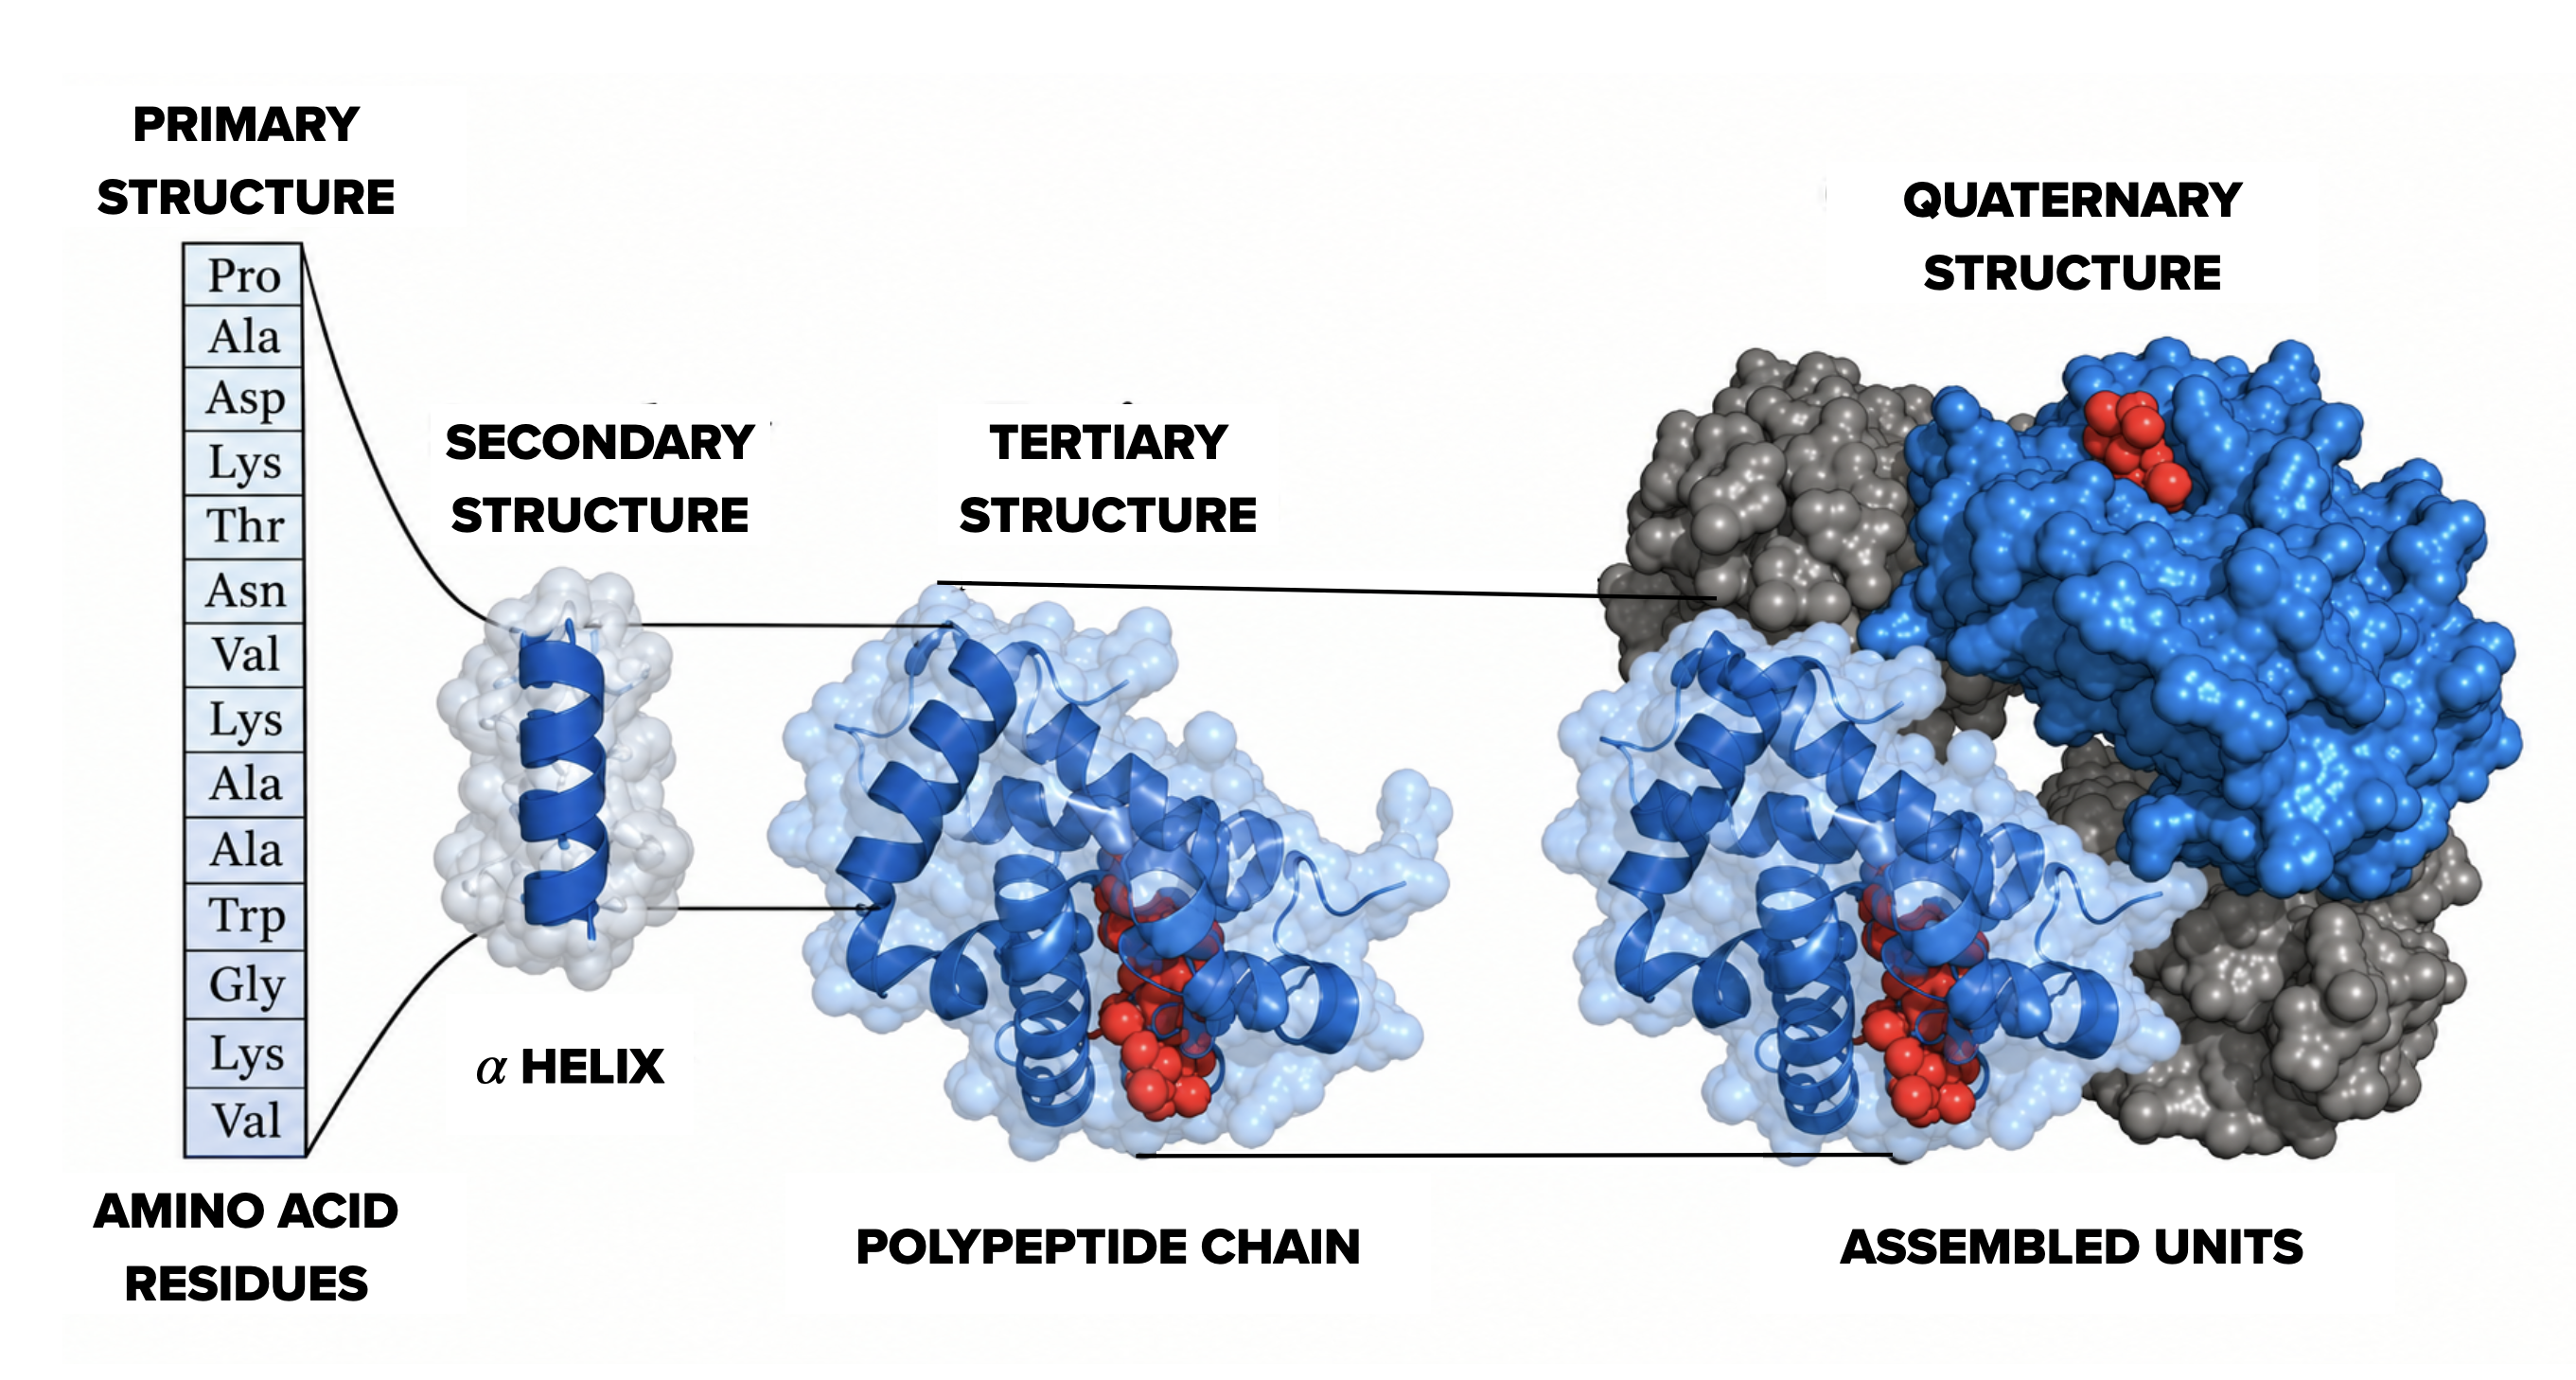
\includegraphics[width=0.9\linewidth]{Protein_intro_figure_high_res.png}
  \caption{\textbf{The four levels of protein structure.} The amino-acid sequence
    (primary structure) folds locally into elements such as $\alpha$-helices
    (secondary structure), which pack into the fold of a single polypeptide chain
    (tertiary structure); several chains then associate through non-covalent
    interfaces into an assembly of subunits (quaternary structure). Adapted from
    \textcite{rashid_protein_2015}.}
  \label{fig:protein-structure}
\end{figure}

The quaternary level is the one this work addresses. A symmetric assembly is
generated by applying the rotations of a point group to a repeating unit called
the \emph{asymmetric subunit} (ASU). The point groups that close into a finite
assembly are the cyclic groups $C_n$, the dihedral groups $D_n$ and the three
polyhedral groups: tetrahedral $T$, octahedral $O$ and icosahedral $I$, of order
$12$, $24$ and $60$ respectively (Figure~\ref{fig:symmetries}). The order of the
group fixes how many copies of the ASU the particle contains. Helical symmetry,
 is the one case that does not close: it repeats the
subunit along a screw axis to give an open filament rather than a bounded
particle. For all these classes of symmetric proteins, the chains within an 
ASU need not be identical. Where the ASU is a single chain the assembly is a symmetric
homo-oligomer, but placing two or more distinct chains in the ASU gives a
multi-component particle.

\begin{figure}[t]
  \centering
  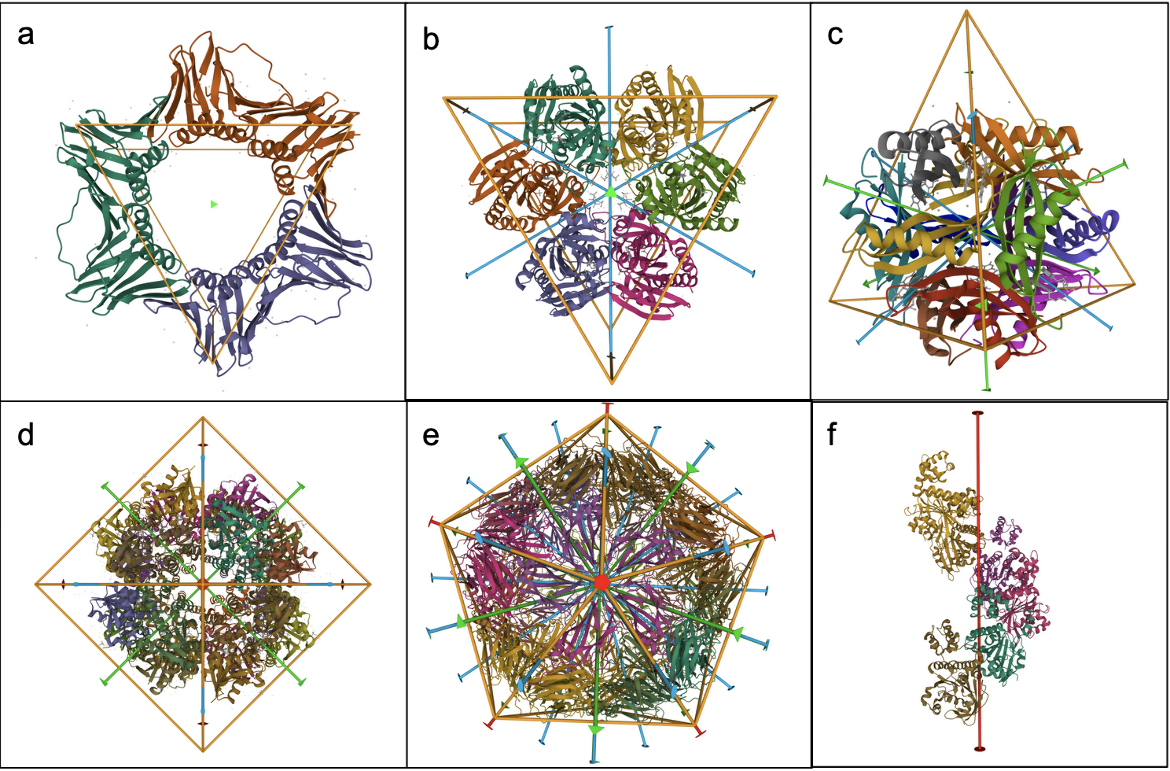
\includegraphics[width=0.92\linewidth]{protein_symmetries.png}
  \caption{\textbf{Symmetry in protein assemblies.} Representative structures
    with their rotation axes drawn.
    \textbf{(a)} Cyclic $C_3$: human PCNA (PDB~3JA9).
    \textbf{(b)} Dihedral $D_3$: \emph{P.~falciparum} purine nucleoside
    phosphorylase (PDB~1NW4).
    \textbf{(c)} Tetrahedral $T$: \emph{H.~salinarum} dodecin (PDB~1MOG).
    \textbf{(d)} Octahedral $O$: phosphopantetheine adenylyltransferase
    (PDB~6CHL).
    \textbf{(e)} Icosahedral $I$: satellite tobacco necrosis virus (PDB~1STM).
    \textbf{(f)} Helical: Rad51 filament (PDB~6DJO).
    Adapted from \textcite{rcsb_symmetry}.}
  \label{fig:symmetries}
\end{figure}

\subsection{Transformers and attention}
\label{subsec:transformers}

A transformer \parencite{vaswani_attention_2017} is a neural network composed of
repeated blocks. It operates on a set of $n$ \emph{tokens}, each carrying a
feature vector of width $d$. To give an example, in the models used in this
report a token corresponds to a residue or an atom.

The original architecture stacks two kinds of block. An encoder block holds a
self-attention sub-layer followed by a position-wise feed-forward sub-layer. A
decoder block adds a third sub-layer, which attends over the encoder output, and
masks its own self-attention so that a position cannot attend to later ones.
Every sub-layer in either kind is wrapped in the same way: its output is added
back to its input through a residual connection, and the sum is layer-normalised.
Architectures that followed, including the protein design model used in this report,
have expanded the same basic structure of the encoder block here described.

\begin{figure}[t]
  \centering
  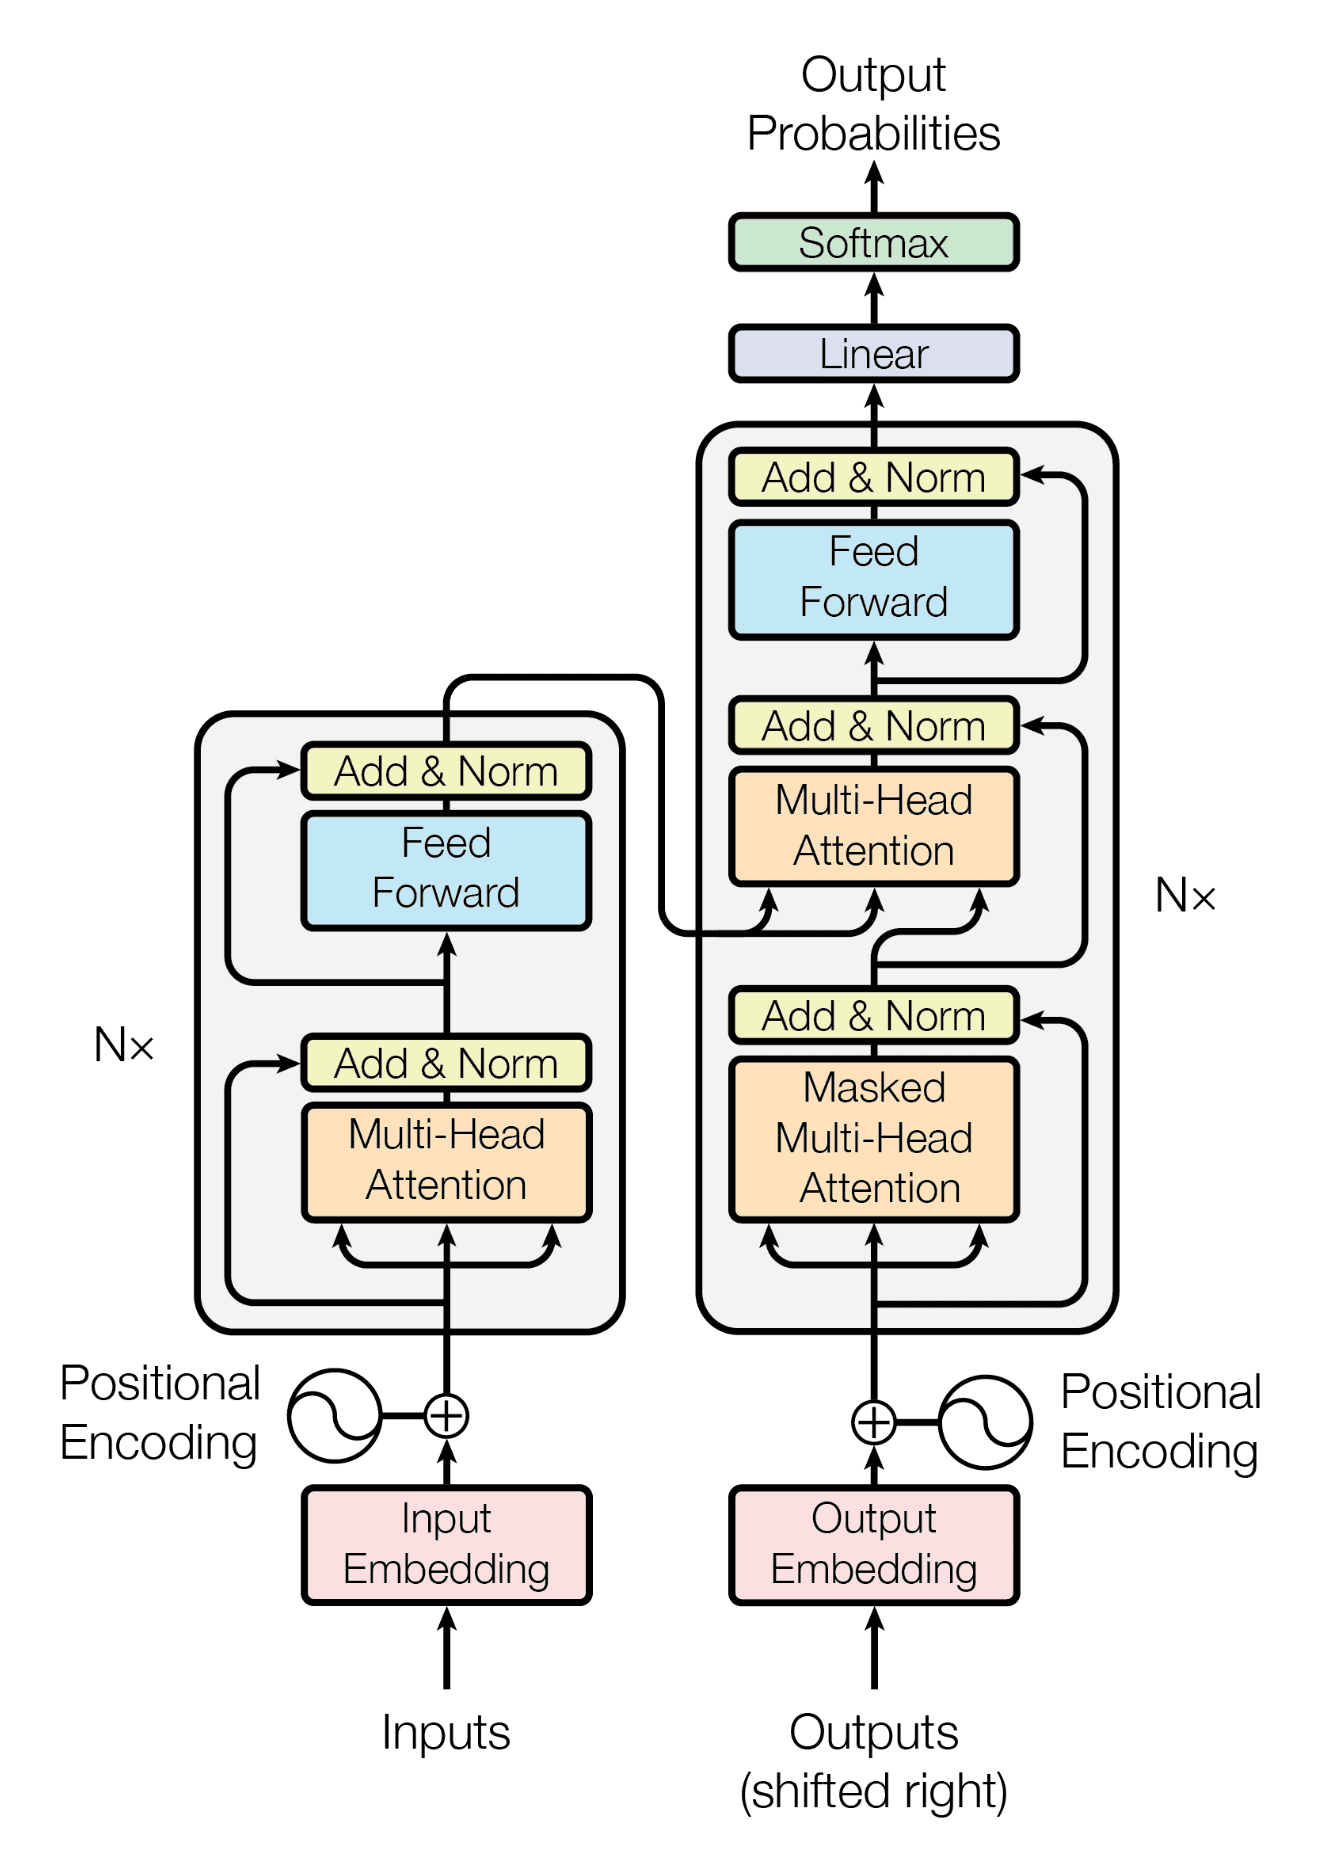
\includegraphics[width=0.55\linewidth]{transformer_architecture.png}
  \caption{\textbf{The original transformer architecture.} The encoder stack is
    on the left and the decoder stack on the right, each repeated $N$ times. An
    encoder block pairs multi-head self-attention with a feed-forward sub-layer;
    a decoder block masks its self-attention and inserts a second attention
    sub-layer that reads the encoder output. Each sub-layer is followed by an
    \textsf{Add \& Norm} step, which is the residual connection and the layer
    normalisation. The embeddings, the positional encodings and the final linear
    and softmax head belong to the sequence-to-sequence task of the original work
    rather than to the block itself. Reproduced from
    \textcite{vaswani_attention_2017}.}
  \label{fig:transformer}
\end{figure}

A block therefore updates each token with a revised feature vector. The attention 
mechanism allows each token to consider the context provided by all other tokens 
in the sequence. The update applied to one
token is a learned, weighted combination of contributions from every other token,
so that a residue can come to be represented in terms of the residues it sits
against rather than by its own identity alone. The feed-forward sub-layer, in
contrast, is applied to each token separately and identically, and the residual
connection and the normalisation likewise act on one token at a time; attention
is therefore the only operation in the block through which tokens exchange
information.

Figure~\ref{fig:attention} sets out the mechanism for a single head. After collecting the
input tokens as the rows of $X \in \mathbb{R}^{n \times d}$, three learned
projections turn each token into a query, a key and a value,
%
\[
  Q = X W_Q^{\top}, \qquad K = X W_K^{\top}, \qquad V = X W_V^{\top},
\]
%
with $Q, K \in \mathbb{R}^{n \times d_k}$ and $V \in \mathbb{R}^{n \times
d_v}$. Every query is scored against every key, and a row-wise softmax turns
those scores into the attention matrix
%
\[
  A = \mathrm{softmax}\!\left(\frac{QK^{\top}}{\sqrt{d_k}}\right)
  \in \mathbb{R}^{n \times n},
\]
%
whose $i$th row holds the weights that token $i$ assigns to each token in the
set. Dividing by $\sqrt{d_k}$ keeps the scores in a range where the softmax does
not saturate. The output of the head is $Z = AV$: every token is replaced by a
weighted average of the values, the weights being those learned scores. Several
such \emph{heads} can operate in parallel on different projections of the same
input (not shown in the image); their outputs are concatenated and mapped back to width $d$ by a further
learned projection, and the result enters the residual connection and the
normalisation described above.

\begin{figure}[t]
  \centering
  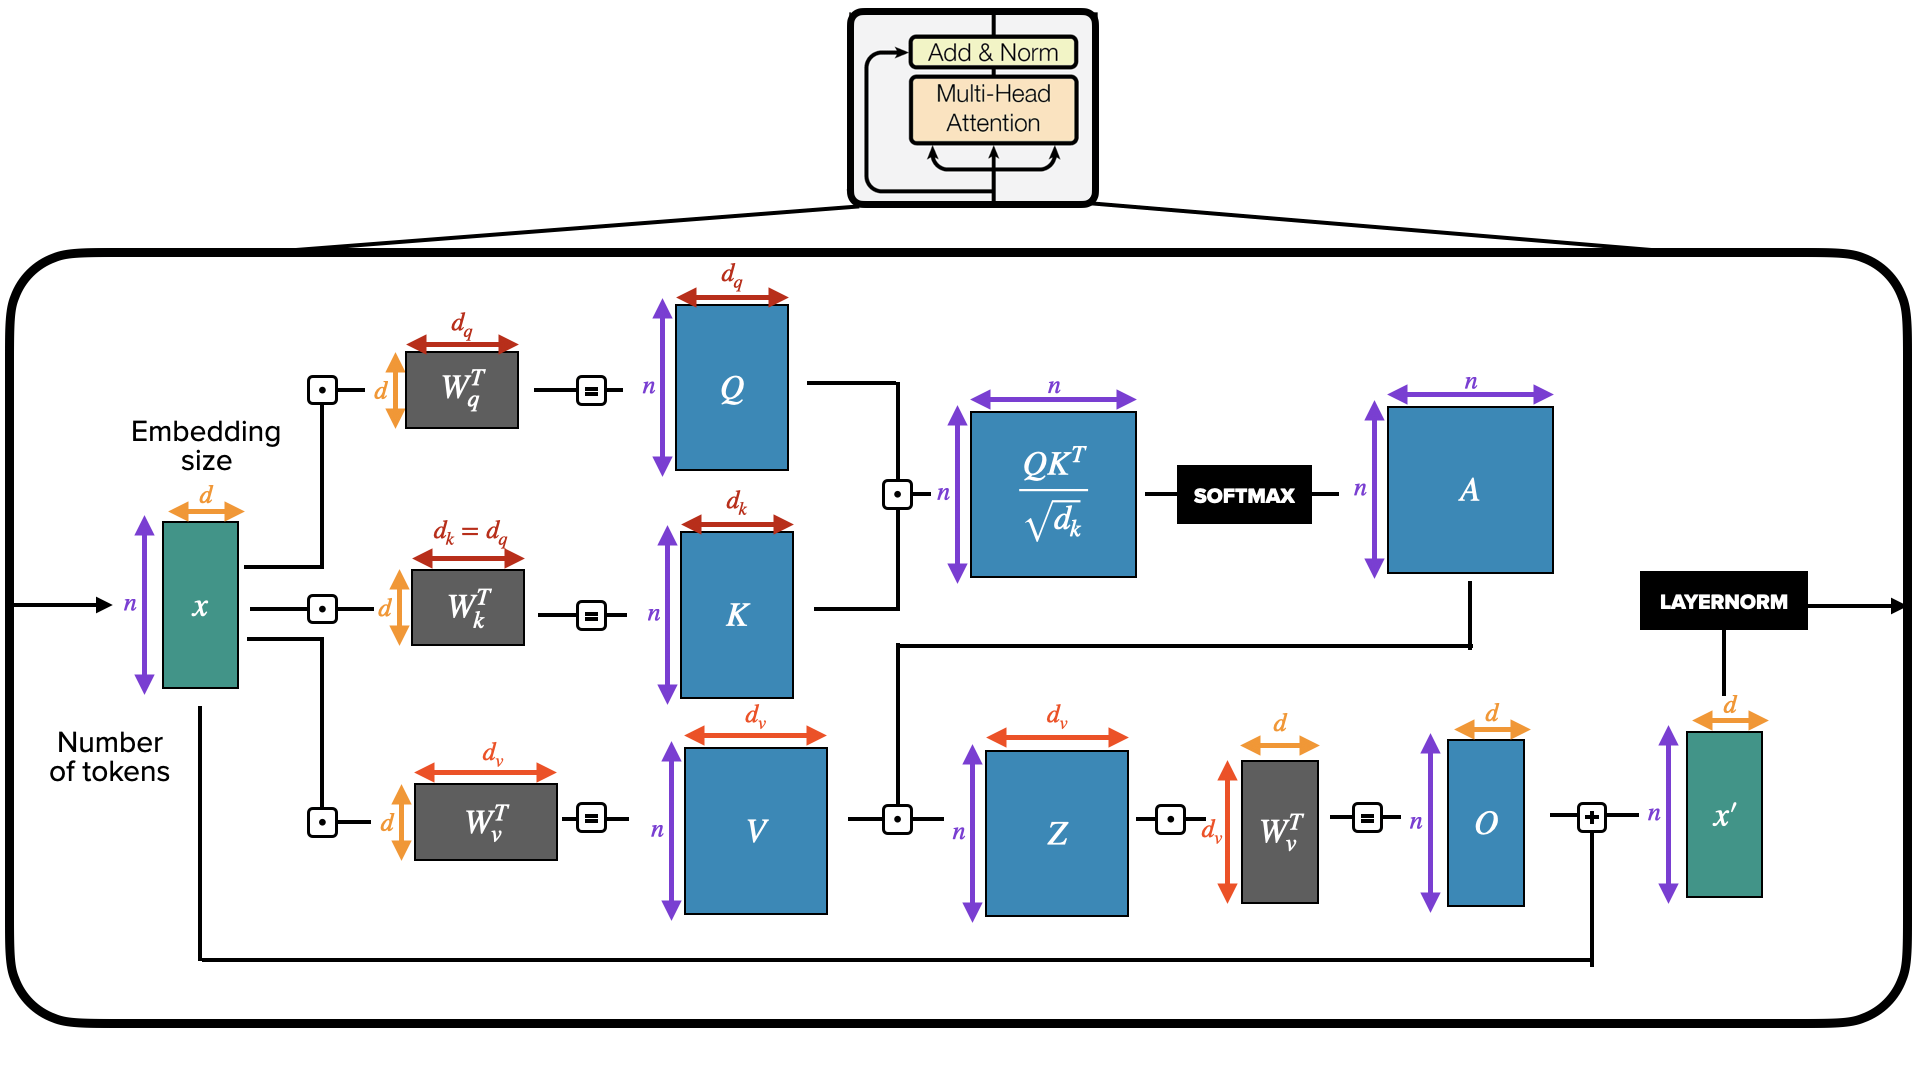
\includegraphics[width=\linewidth]{Attention.png}
  \caption{\textbf{One attention sub-layer, unrolled.} The multi-head attention
    block at the top is reproduced from the original transformer paper
    \parencite{vaswani_attention_2017}; the panel below expands it for a single
    head and includes the residual connection and the layer normalisation that
    close the sub-layer. Tensors are shaded by role and annotated with their
    dimensions; the symbols are those used in the text.}
  \label{fig:attention}
\end{figure}

The meory cost associated with this vanilla implementation is quadratic in the sequence length. 
Since every token is scored against every other, the scores form an $n\times n$ matrix, so an
attention layer requires $\mathcal{O}(n^2)$ time, and materialising that matrix
requires $\mathcal{O}(n^2)$ memory. On top of this, models that predict or generate the
structure of proteins often introduce a second quadratic object, a \emph{pair representation} holding one
feature vector for every pair of tokens. The attention matrix is formed and
discarded within a single layer, whereas the pair representation is maintained and
updated throughout the network and must therefore be held in memory for the entire
forward pass. We describe in more details this issue and our solution to it in Chapter~\ref{ch:methods}.
%These two quadratic terms are the reason large assemblies are
%expensive to model, and Chapter~\ref{ch:methods} distributes them across several
%GPUs.

\section{Protein nanoparticle vaccines}
\label{sec:pnp-vaccines}

The clinical success of mRNA vaccines during the SARS-CoV-2 pandemic
\parencite{polack_safety_2020} established nucleic-acid delivery as a fast,
programmable vaccine modality: manufacture is sequence-independent and scalable
\parencite{pardi_mrna_2018}, and clinical-grade material for mRNA-1273 entered
production five days after the SARS-CoV-2 sequence was released, reaching a
phase~1 trial 66 days later \parencite{corbett_sars-cov-2_2020}. This platform 
has, however, innately limited immunogenicity. An antigen presented as a
soluble monomer is often only weakly immunogenic, because the size, geometry and
repetitiveness with which an antigen is displayed largely govern how strongly it
engages the immune system \parencite{bachmann_vaccine_2010}.

A complementary strategy is therefore to present the antigen not as a soluble
monomer but arrayed on the surface of a self-assembling \emph{protein
nanoparticle}, in many copies and in a dense, repetitive, virus-like geometry
(Figure~\ref{fig:pnp-vaccine}).
Designed nanoparticle vaccines of this kind have elicited neutralising-antibody
responses roughly an order of magnitude stronger than the corresponding soluble
antigen, both for SARS-CoV-2
\parencite{walls_elicitation_2020} and for respiratory syncytial virus
\parencite{marcandalliInductionPotentNeutralizing2019a}; in the SARS-CoV-2 case
the titres were still undiminished twenty weeks after the boost. The same
principle of geometry-matched multivalent display also underpins designed
miniprotein inhibitors, which neutralise variants of concern and protect mice
when given intranasally before or after challenge
\parencite{hunt_multivalent_2022}. Natural and engineered self-assembling
scaffolds such as lumazine synthase provide versatile platforms for multivalent,
cross-protective antigen presentation
\parencite{ladenstein_second_2020,joseph_lumazine_2025}, and self-assembling
protein nanoparticles are now engineered both for therapeutic delivery
\parencite{olshefskyEngineeringSelfAssemblingProtein2022} and as modular nanocages that
display antibodies and Fc fusions at controlled valency, a format that enhances
receptor agonism and viral neutralisation \parencite{divine_designed_2021}.\\

\begin{figure}[t]
  \centering
  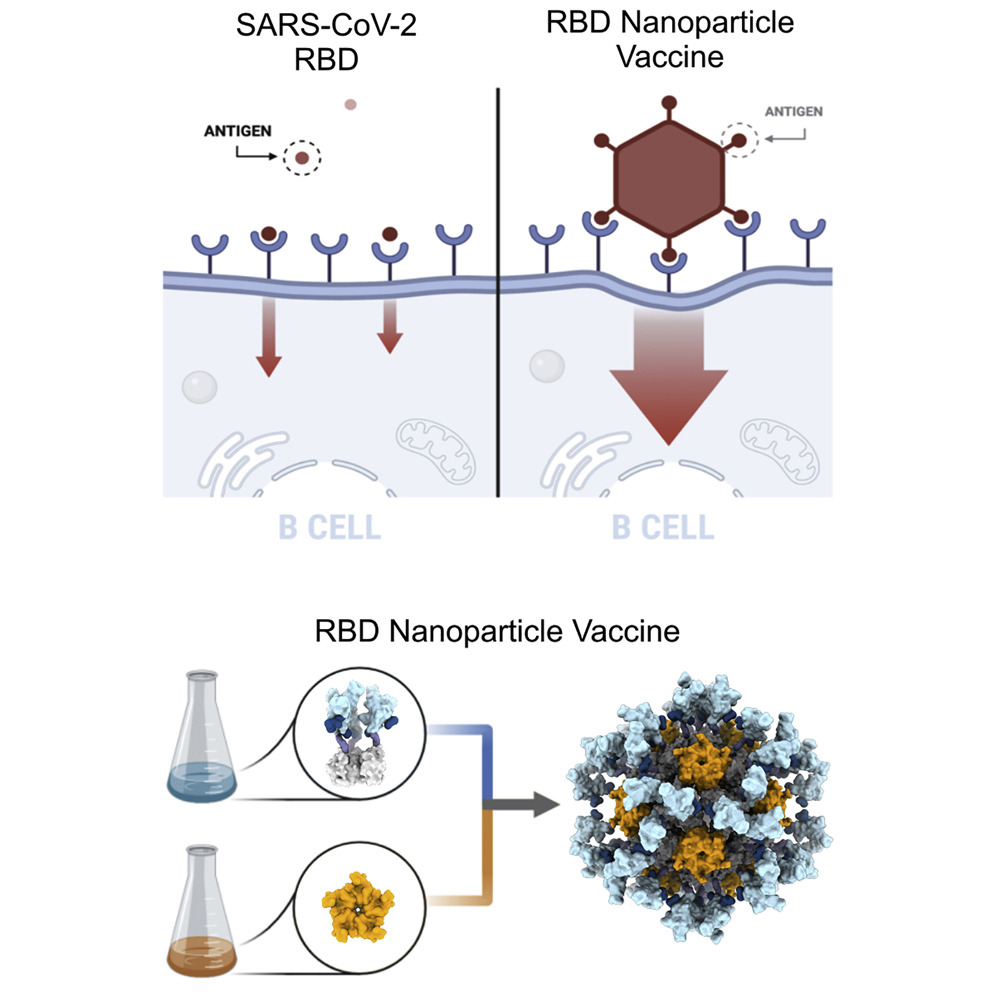
\includegraphics[width=0.58\linewidth]{Protein_nanoparticle_vaccine.jpg}
  \caption{\textbf{Antigen display on a designed nanoparticle.} \textbf{Top:} a
    soluble SARS-CoV-2 receptor-binding domain engages few B-cell receptors,
    whereas the same antigen displayed in sixty copies on a nanoparticle engages
    many at once and elicits a far stronger response. \textbf{Bottom:} the
    scaffold is two-component, a trimer bearing the antigen and a pentamer, which
    are expressed separately and co-assemble into the icosahedral particle.
    Reproduced from \textcite{walls_elicitation_2020}.}
  \label{fig:pnp-vaccine}
\end{figure}

Crucially, because the scaffold is itself a protein, the nanoparticle and its
displayed antigen can be genetically encoded and delivered as a single mRNA
construct, so that the immunogen self-assembles \emph{in vivo}. This
``mRNA-launched'' route combines the manufacturing speed of nucleic-acid vaccines
with the superior immunogenicity of particulate display, and computationally
designed mRNA-launched nanoparticle immunogens have been shown to elicit
protective antibody and T-cell responses in mice
\parencite{hendricks_computationally_2025}. The vaccine platform we target in this
work is therefore \emph{fully protein based}: making it a design target that, as we argue in
Chapter~\ref{ch:comp-design}, can be tackled with modern generative protein models.


% Suggested figure: a schematic contrasting (i) soluble antigen, (ii) nanoparticle
% display, and (iii) mRNA-launched self-assembly. Drop the file in figures/ and
% uncomment.
% \begin{figure}[t]
%   \centering
%   \includegraphics[width=\linewidth]{fig_nanoparticle_vaccine_schematic.pdf}
%   \caption{From soluble antigen to mRNA-launched nanoparticle display.}
%   \label{fig:pnp-schematic}
% \end{figure}


\section{Protein design}
\label{sec:protein-design}

Designing the scaffolds described above is a protein-design problem: we must
specify an amino-acid sequence that folds into, and assembles into, 
a prescribed three-dimensional architecture. This section sketches how the field 
of protein design in general has moved from
physics-based methods to today's machine-learning approaches.

\subsection{Physics-based design}
\label{subsec:physics-design}

The first generation of computational protein design was grounded in biophysics:
candidate sequences were threaded onto a target backbone and scored with an
energy function approximating the physics of folding, with the conformational and
sequence search handled by algorithms such as those in the Rosetta suite. This
paradigm produced landmark results, including the first de novo globular fold
designed to atomic-level accuracy \parencite{kuhlman_design_2003}, de novo enzymes
for reactions with no natural catalyst
\parencite{rothlisberger_kemp_2008,siegel_computational_2010} and picomolar
miniprotein inhibitors of SARS-CoV-2 \parencite{cao_novo_2020}.

For assemblies, symmetry was built into the method itself. The earliest approach
fused two natural oligomers through a rigid helical linker, so that the symmetry
of each component fixed the geometry of the whole
\parencite{padilla_nanohedra_2001}. It gave way to the two-stage recipe that has
defined the field since: rigid-body docking of symmetric building blocks into a
target architecture, followed by atomic-level design of the interfaces this
creates between them. The recipe produced self-assembling nanomaterials whose
crystal structures matched the design models
\parencite{king_computational_2012}, and went on to yield co-assembling
multi-component materials \parencite{king_accurate_2014}, megadalton-scale
two-component icosahedra \parencite{bale_accurate_2016} and hyperstable
60-subunit cages \parencite{hsia_design_2016}, with fast sequence-independent
docking software making the pose search practical
\parencite{sheffler_fast_2023}. These methods work, but they are bounded by their building blocks: docking
draws only on oligomers that already exist, each of which must then be
repurposed, with a new interface designed onto a surface that evolved for
something else. %TO

\subsection{The machine-learning revolution in de novo design}
\label{subsec:ml-design}

The accuracy revolution in protein \emph{structure prediction} that includes AlphaFold2
\parencite{jumperHighlyAccurateProtein2021}, RoseTTAFold
\parencite{baekAccuratePredictionProtein2021} and, more recently, the all-atom
biomolecular model AlphaFold3 \parencite{abramsonAccurateStructurePrediction2024} transformed what is computationally tractable, and it was quickly followed by an
analogous revolution in \emph{generative} design. Deep generative models now propose novel structures directly. Denoising-based
design frameworks including RFdiffusion \parencite{watsonNovoDesignProtein2023},
Chroma \parencite{ingrahamIlluminatingProteinSpace2023} and Genie
\parencite{lin_generating_2023,lin_out_2024,linFastUltraCapableProtein2026},
together with the flow-based Proteina \parencite{geffner_proteina_2025}, enable
the de novo creation of proteins with prescribed structural and functional
properties. Most generate a backbone alone, and their sequences are supplied by a
learned inverse-folding model such as ProteinMPNN
\parencite{dauparasRobustDeepLearning2022}; Chroma instead designs sequence and
side chains for whole complexes itself, and the recent RFdiffusion3
\parencite{butcher_novo_2025}, on which this work builds, generates every atom.

The reach of this toolkit is clearest in what it has been used to make: de novo
minibinders against therapeutically relevant targets, from bioactive peptide
hormones \parencite{vazquez_torres_novo_2024} to clostridial toxins
\parencite{ragotte_novo_2025}; epitope-targeted antibodies, from diffusion-based
co-design of complementarity-determining regions on a fixed framework
\parencite{luo_antigen-specific_2022} to atomically accurate designs of VHHs and
scFvs \parencite{bennett_atomically_2026}; and de novo enzymes
\parencite{yeh_novo_2023}. Recent reviews chart the trajectory of the field
\parencite[e.g.][]{yang_past_2026}.

Two threads run through this chapter: a vaccine platform that is entirely protein
based, and a design toolkit that no longer depends on parts borrowed from nature.
Chapter~\ref{ch:comp-design} brings them together and sets out what still stands
between them and a designed nanoparticle vaccine.

%==============================================================================
% Chapter 2 -- Computational design of protein nanoparticle vaccines
%==============================================================================
\chapter{Computational design of protein nanoparticle vaccines}
\label{ch:comp-design}

% -----------------------------------------------------------------------------
% This chapter expands the "Computational design of protein nanoparticles"
% thread of the Design-CP paper's Related Work into a proper background section,
% and then states the objective of the project. It is the pivot of the report:
% it sets up why modelling the *whole assembly* end to end is the enabling first
% step, which is exactly the premise of the Design-CP work reported in
% Chapters 3-4.
% -----------------------------------------------------------------------------

\section{Current methods}
\label{sec:current-methods}

State-of-the-art design of protein nanoparticles follows a two-stage
``dock-and-design'' recipe inherited from the Rosetta era. First, symmetric
oligomeric building blocks are rigidly docked into a target point-group
architecture (for example a tetrahedron, octahedron or icosahedron) so that their
symmetry axes coincide with those of the target; second, the newly created
subunit--subunit interfaces are redesigned to drive stable self-assembly. This
programme produced the first self-assembling protein nanomaterials with
atomic-level accuracy \parencite{king_computational_2012}, its multi-component
extension \parencite{king_accurate_2014}, megadalton-scale two-component
icosahedral complexes such as I53-50 \parencite{bale_accurate_2016} and the
hyperstable 60-subunit icosahedron I3-01 \parencite{hsia_design_2016}, building on
symmetric self-assembly principles established earlier
\parencite{padilla_nanohedra_2001}. Machine learning has since accelerated the
generation of building blocks and the design of interfaces: symmetric assemblies
have been produced by hallucination
\parencite{wickyHallucinatingSymmetricProtein2022}, interfaces are now routinely
designed with ProteinMPNN \parencite{de_haas_rapid_2024}, and the building blocks
themselves are drawn from AlphaFold2-predicted structures
\parencite{haas_sequence_2025} or generated de novo with RFdiffusion
\parencite{haas_novo_2026}. Related advances extend the repertoire to
pseudosymmetric and multi-component cages
\parencite{dowlingHierarchicalDesignPseudosymmetric2025,
rankovicComputationalDesignBifaceted2025,lee_four-component_2025,kibler_design_2024}.

Despite this progress, essentially all of these pipelines share a structural
limitation: they still rely on a \emph{rigid-body docking step} over a library of
pre-computed oligomers. The building blocks are designed, or predicted, in
isolation and are only afterwards assembled by a search over rigid poses. The
inter-subunit interfaces---the very interactions that determine whether, and how
well, a particle assembles---are therefore never generated jointly with the rest
of the structure. A natural next step is to remove the docking stage altogether
and model the entire assembly, including all of its inter-subunit interfaces, with
a single generative network.


\section{Objective of our project}
\label{sec:objective}

The objective of this project is to marry the fully protein-based nanoparticle
vaccine platform of Chapter~\ref{ch:introduction} with the generative-modelling
capabilities of Chapter~\ref{sec:protein-design}: to design protein nanoparticle
vaccines \emph{end to end}, as whole assemblies, with a single all-atom generative
model rather than a docking pipeline over independently designed parts. In the
longer term (Chapter~\ref{ch:future-work}) this means \emph{conditional} design---
scaffolding a chosen antigen onto a self-assembling particle---but that ambition
rests on a prerequisite that turns out to be non-trivial.

\paragraph{The enabling first step: modelling the whole assembly.}
Before one can condition generation on a displayed antigen, one must first be able
to \emph{model the whole assembly at all}. All-atom generative models can, in
principle, design a large multimeric complex by jointly denoising every chain and
every atom; in practice, their quadratic token-pair and atom-pair representations
exhaust the memory of a single GPU as the number of subunits and residues grows.
A full icosahedral particle---sixty chains and many thousands of residues---simply
does not fit. This memory ceiling is the reason the field still falls back on
docking pre-computed oligomers rather than generating the assembly directly.

This report addresses exactly that bottleneck. Building on the all-atom model
RFdiffusion3 \parencite{butcher_novo_2025}, we borrow \emph{context parallelism}
from large-language-model and structure-prediction systems
\parencite{lin_fold-cp_2026,dao_flashattention_2022} to distribute the quadratic
activations across a multi-GPU mesh, so that the full assembly can be denoised in a
single trajectory. The result---presented in Chapters~\ref{ch:methods}
and~\ref{ch:results}---is, to our knowledge, the first end-to-end, all-atom
generative design of symmetric protein assemblies that models the full set of
inter-subunit interactions without an intermediate docking step. Establishing that
we can reliably model the whole assembly is the premise on which every subsequent
research direction in this report is built.

\chapter{Current Memory Reduction Methods}
\label{ch:current-memory-reduction-methods}

Recent all-atom generative models such as RFDiffusion 3~\cite{butcher_novo_2025} (RFD3), 
which is inspired by the AlphaFold 3 architecture~\cite{abramson_accurate_2024} (AF3),
can in principle generate multimeric structures such as the symmetric assembly needed as scaffolds
for nanoparticle vaccines. This is achieved by jointly modelling all chains with
an atomistic level of precision and designing proteins with predefined point-group 
symmetries. However, the underlying architecture maintains pairwise representations 
whose memory cost scales quadratically with the number of tokens~$I$ (and atoms~$L$). 
For protein assemblies, $I$ and $L$ grow linearly with the number of chains
modelled, causing the $\mathcal{O}$($I^{2}$) and $\mathcal{O}$($L^{2}$) pairwise 
feature tensors and related quadratic intermediates to exceed the memory capacity 
of a single GPU when trying to model assemblies of the size relevant for nanoparticle vaccines. 
This practical bottleneck therefore heavily limits the size of what can be
designed.

% This single-device ceiling, however, contrasts with broader trends in 
% computational infrastructure: while single-device memory capacity has grown only 
% incrementally, access to multi-GPU clusters is now routine for both academic and 
% industrial research groups. Accordingly, partitioning large transformer workloads 
% across such clusters has become standard practice in adjacent fields such as large 
% language modelling, both for training~\cite{li_sequence_2022} and 
% inference~\cite{pope_efficiently_2022}.

\section{Reducing the cost of attention}
\label{sec:reducing-attention-cost}

In the literature (especially in the one related to large language models), several strategies have 
been proposed to reduce the memory cost of attention. Here we briefly cover 
IO-efficient attention on a single device, while devoting most of this sec-
tion to distributed parallelism for structure models, because our developed solution 
\cref{ch:methods} sits in this realm. 

\subsection{IO-efficient attention}
\label{subsec:io-efficient-attention}
FlashAttention \cite{dao_flashattention_2022, dao_flashattention-2_2023}
computes exact attention with memory linear in sequence length 
($\mathcal{O}(I)$ or $\mathcal{O}(L)$ in our notation) by tiling queries, keys, 
and values into SRAM-resident blocks while maintaining running softmax statistics 
\citep{milakov_online_2018}, building on the earlier observation that attention 
admits a linear-memory implementation \citep{rabe_self-attention_2022}. 
For architectures without pair representations, this suffices and motivates its 
use in protein language models like ESM3 \citep{hayes_simulating_2025}, which 
represent sequence, structure, and function as discrete tokens and condense 
pairwise geometry into a single SE(3)-invariant geometric-attention block at 
the input. Flash‑IPA \citep{liu_flash_2025} and FlashBias \citep{wu_flashbias_2025} 
extend this idea to pair‑biased attention, such as the one present in AlphaFold‑3 
Pairformer, by re-expressing geometric and pairwise bias terms via additional low‑rank 
features concatenated into the query and key projections. For complex learned pair
biases, these methods generally require training auxiliary parameters and are not 
a weight‑preserving drop‑in for an arbitrary pretrained model. 
% These approaches are 
% orthogonal to Design-CP: they reduce the per-block memory footprint on a single device, 
% while we shard the persistent quadratic activations across devices, and the two could in principle be composed.

\subsection{Distributed parallelism for structure models.} 
Among the standard parallelism axes (data, tensor, pipeline, expert, activation), 
\emph{context parallelism} uniquely shards activations along the sequence dimension 
of every layer, which makes it a natural fit for the $\mathcal{O}(I^2)$ pair tensor 
of AlphaFold-class models. FastFold \citep{cheng_fastfold_2023} introduced Dynamic 
Axial Parallelism (DAP) for AlphaFold~2, replicating parameters on every device and 
sharding activations along a single sequence axis at a time; 
ScaleFold \citep{zhu_scalefold_2024} adopted DAP and scaled to 2048 H100s for training. 
As the Evoformer interleaves row- and column-wise attention over the MSA track, 
DAP must insert an all-to-all communication step whenever the active axis flips, 
incurring six all-to-all redistributions per Evoformer block at inference, together
with one \textsc{AllGather} in the outer-product-mean and two in the triangular
updates~\citep{cheng_fastfold_2023}. These collectives contribute non-trivially 
to inference latency at scale and increase transient memory relative to the 
steady-state ($\mathcal{O}(I^2/P)$, where $P$ is the total number of devices) sharded pair representation.

Fold-CP \citep{lin_fold-cp_2026} generalises axis sharding to a full two-dimensional 
context-parallel strategy for AF3-class models (implementing it for 
Boltz-2~\citep{passaro_boltz-2_2025}), extending Ring Attention~\citep{liu_ring_2023} 
into a Cannon-style 2D ring tailored to dense triangular updates, while window-batched
atom attention is handled by a complementary shardwise kernel that keeps each 
window's attention local to its rank. The pair tensor is tiled over a 
$\sqrt{P}\times\sqrt{P}$ device grid, so that rank $(r,c)$ holds the block indexed 
by residue ranges $[r\cdot I/\sqrt{P}, (r{+}1)\cdot I/\sqrt{P}]\times [c\cdot I/\sqrt{P}, (c{+}1)\cdot I/\sqrt{P}]$. 
Triangle attention, triangle multiplication, attention-with-pair-bias, pair-weighted-averaging, 
and outer-product-mean are each reformulated as ring algorithms in which $\mathbf{K}$ 
and $\mathbf{V}$ shards (and, where required, triangular biases and masks) circulate 
between neighbouring devices while a numerically-stable tiled softmax merges partial 
outputs without ever materialising the full $I\times I$ attention on any rank. 
The resulting steady-state pair memory per device is ($\mathcal{O}(I^2/P)$), matching 
1D axis-sharded DAP. However, under 1D sharding, triangular updates typically require 
collectives over all ($P$) ranks (e.g., to obtain the necessary key/value or bias 
shards along the active axis), which can inflate the transient working-set memory 
during attention/multiplication beyond the steady shard. In Fold‑CP’s 2D tiling, 
collectives are restricted to a single row or column subgroup of size ($\sqrt{P}$). 
This reduces communication volume and confines the transient working-set memory growth
in triangular updates (e.g., gathered/circulated K/V shards, triangle biases, masks,
and other pair-like intermediates) to ($\sqrt{P}$)-sized groups, rather than requiring 
global ($P$)-way collectives.

%==============================================================================
% Chapter 3 -- Methods
%==============================================================================
\chapter{Methods}
\label{ch:methods}

% -----------------------------------------------------------------------------
% Adapted from Section 3 of the Design-CP paper. This is the technical core of
% the report and (as in the example) the longest chapter. Verify every numerical
% constant and symbol against the paper before submission; where the paper's
% appendices give more detail (device meshes, communication volumes), summarise
% here and cite the appendix.
% -----------------------------------------------------------------------------

As discussed in Chapter~\ref{ch:current-memory-reduction-methods}, the current barrier for designing
whole protein assembly de-novo is a memory problem. An all-atom
generative model can express a whole assembly, but cannot hold its quadratic
activations needed for pair-biased attention on one accelerator. This chapter introduces \emph{Design-CP}, two
context-parallel inference strategies that shard those activations across a
multi-GPU mesh while leaving the pretrained model weights untouched. Neither
scheme alters the computation the model performs: both reproduce single-GPU
inference numerically, and only the placement of the activations across devices
differs.

\section{RFdiffusion3 preliminaries and notation}
\label{sec:rfd3-prelim}

We build on RFdiffusion3 (RFD3) \parencite{butcher_novo_2025}, an all-atom denoising-diffusion model whose
diffusion module follows the AlphaFold3 design
\parencite{abramsonAccurateStructurePrediction2024} and which is
built on the AtomWorks framework \parencite{corley_accelerating_2025}. At each denoising step RFD3 jointly represents a
structure at two resolutions. A \emph{token} track carries a single
representation $S \in \mathbb{R}^{I \times c_s}$ and a pair representation
$Z \in \mathbb{R}^{I \times I \times c_z}$ over $I$ tokens; an \emph{atom} track
carries a single representation $A \in \mathbb{R}^{L \times c_\text{atom}}$ and a pair representation
$P \in \mathbb{R}^{L \times L \times c_\text{atompair}}$ over $L$ atoms. Attention
on each track adds a learned pair bias to the logits, e.g.
%
\begin{equation}
  \mathrm{Attn}(S) = \mathrm{softmax}\!\left(\frac{QK^\top}{\sqrt{d}} + B(Z)\right)V,
  \label{eq:pair-bias-attn}
\end{equation}
%
where $B(Z) \in \mathbb{R}^{I \times I \times H}$ projects the pair track into a
bias for each of the $H$ attention heads. Atom attention can be made \emph{sparse}
using a $k$-nearest-neighbour neighbourhood with $k \ll L$, so its compute cost is
$\mathcal{O}(Lk)$ rather than $\mathcal{O}(L^2)$. This is an approximation with respect to 
how the model was trained (which used the full matrix $P$), and when not used the pair storage $P$
remains quadratic in $L$. The single-GPU memory footprint is
therefore dominated by the $\mathcal{O}(I^2)$ and possibly the $\mathcal{O}(L^2)$ pair tensors,
which is what limits the size of assembly that can be modelled at once.
Sampling follows the EDM framework \parencite{karras_elucidating_2022} with the
AlphaFold3 schedule. We leave the stock RFD3 settings untouched:
$T=200$ denoising steps, two recycling iterations per step, and a sparse atom
neighbourhood of $k=128$ keys.

When designing with a pre-defined point symmetry, the diffusion model is always
run on the entire complex at every denoising step. For a configurable fraction of
the trajectory (default $90\%$), RFD3 then \emph{resymmetrises} its prediction by
extracting the coordinates of a single asymmetric subunit (ASU) and generating the
remaining copies by applying the point-group operations. The resulting
resymmetrised complex is the state that is fed into the next iteration of the
sampling loop. Because the network still denoises every atom of the assembly, it
can account for the full set of inter-subunit interactions, while the symmetry
constraint couples atom positions across subunits and thereby reduces the
effective degrees of freedom of the design to those of a single ASU. The per-step
procedure is set out in Appendix~\ref{app:implementation}.

\begin{figure}[t]
  \centering
  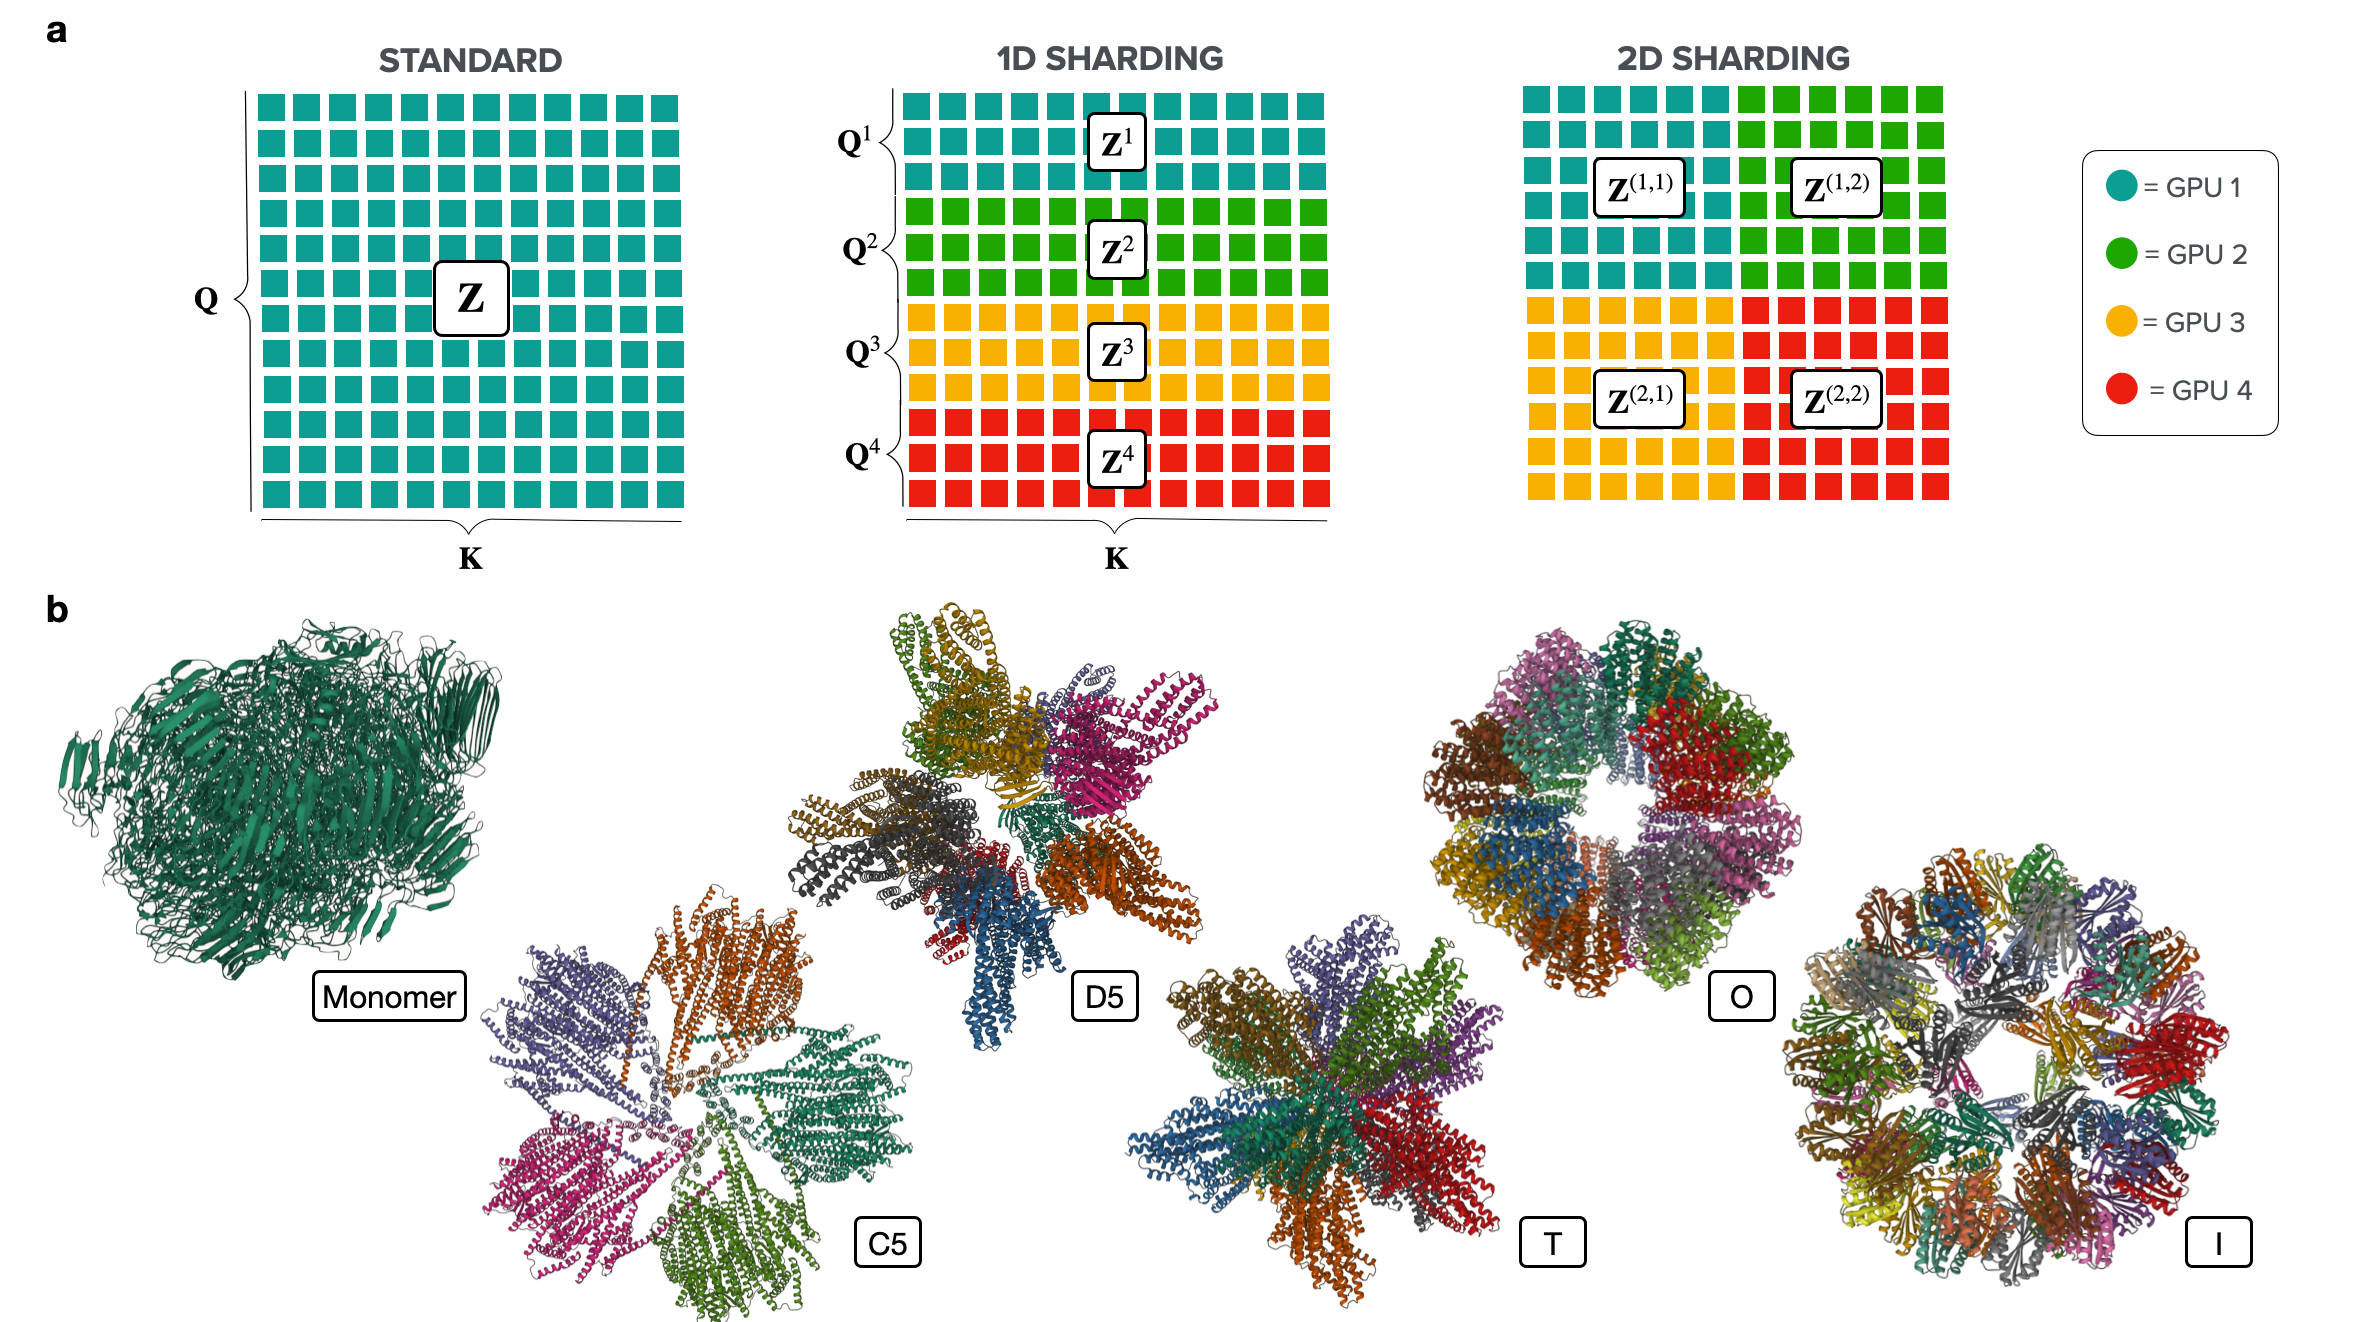
\includegraphics[width=\textwidth]{Figure_1.png}
  \caption{\textbf{Symmetric design with Design-CP.}
    \textbf{(a)} Schematic depiction of the sharding techniques implemented in
    Design-CP. Every square represents a sub-tensor of the self-attention matrix,
    and its colour represents its assigned device. 1D sharding partitions the
    queries across different GPUs, where they are used to calculate
    cross-attention against all keys. 2D sharding partitions both queries and keys
    and uses ring attention to compute attention scores on the fly.
    \textbf{(b)} Qualitative comparison of large-design samples. Designs of a
    $10{,}800$ amino-acid protein using different symmetries. Designs that exceed
    the native crop limits can show visible degradation when sampled without
    additional structure constraints; imposing a strong symmetry prior mitigates
    this effect by reducing the effective design space.}
  \label{fig:large-designs}
\end{figure}

\section{Design-CP 1D row-sharding}
\label{sec:cp-1d}

Our first scheme, implemented in PyTorch with NCCL and without custom kernels or
\texttt{DTensor} machinery, partitions the query dimension of every $I\times I$
and $L\times L$ operation across $P$ GPUs (Figure~\ref{fig:large-designs}a, center).
GPU~$p$ materialises only its row stripe of the pair track:
%
\begin{equation}
  \mathbf{Z}^{(p)} \in \mathbb{R}^{I_p \times I \times c_z}, \qquad
  I_p = \lfloor I/P \rfloor + \mathbb{I}[\,p < I \bmod P\,],
  \label{eq:row-stripe}
\end{equation}
%
where $\mathbb{I}[\,\cdot\,]\in\{0,1\}$ denotes the indicator function of its
predicate. When $I$ is not divisible by $P$, the floor $\lfloor I/P\rfloor$ leaves
a remainder of $I \bmod P$ elements that must still be assigned. We absorb this
remainder by giving the first $I \bmod P$ ranks one additional row each: rank $p$
receives the extra row precisely when $p < I \bmod P$, which is what the indicator
encodes. By construction $\sum_{p}I_p = I$, no element is dropped, and chunk sizes
differ by at most one across GPUs, so the load imbalance per attention block is
bounded by a single row regardless of $P$. The pair tracks $\mathbf{Z}^{(p)}$ and
the self-conditioning distogram $\mathbf{D}^{(p)}_\text{self}$ are in this way
\emph{never} gathered to their full $[I,I]$ shape.

Every self-attention block is reformulated as a cross-attention: GPU~$p$ projects
queries from its stripe $\mathbf{Q}^{(p)}=f_Q(\mathbf{S}^{(p)})\in
\mathbb{R}^{I_p\times H\times d}$, while keys and values are projected from the
\emph{full} single-track $\mathbf{S}$, which is replicated on every GPU. The pair
bias is drawn from the local stripe, $\mathbf{B}^{(p)}=f_B(\mathbf{Z}^{(p)})\in
\mathbb{R}^{I_p\times I\times H}$, and
%
\begin{equation}
  \operatorname{Attn}^{(p)} = \operatorname{softmax}\!\left(
    \mathbf{Q}^{(p)} \mathbf{K}^\top/\sqrt{d} + \mathbf{B}^{(p)}
  \right) \mathbf{V}.
  \label{eq:cross-attn}
\end{equation}
%
A single \textsc{AllGather} over the 1D track reconstructs
$\mathbf{S}=\bigoplus_{p}\mathbf{S}^{(p)}\in\mathbb{R}^{I\times c_s}$ after each
block, so that all GPUs hold identical $\mathbf{K}$ and $\mathbf{V}$ for the next
block. The same partition applies at the atom level. The dense atom pair track is
striped as $\mathbf{P}^{(p)}\in\mathbb{R}^{L_p\times L\times c_\text{atompair}}$,
reducing its per-GPU storage from $\mathcal{O}(L^{2})$ to
$\mathcal{O}(L^{2}/P)$. The sparse $k$-nearest-neighbour attention is then applied
per shard: each GPU gathers, from its stripe of $\mathbf{P}^{(p)}$, the $k$
neighbour entries for each of its $L_p$ query atoms, yielding a local bias
$\mathbf{P}^{(p)}_\text{sparse}\in\mathbb{R}^{L_p\times k\times c_\text{atompair}}$
at attention-computation cost $\mathcal{O}(L\,k/P)$. At diffusion-step boundaries,
rank~$0$ broadcasts the noised coordinates, sampled Gaussian noise and denoised
prediction so that all ranks share a single stochastic trajectory. Per-GPU
pair-track memory is therefore $\mathcal{O}(I^{2}/P)$ for $\mathbf{Z}$ and
$\mathcal{O}(L^{2}/P)$ for $\mathbf{P}$. A more detailed description is provided in
Appendix~\ref{app:implementation}.

\section{Design-CP 2D grid context parallelism}
\label{sec:cp-2d}

Our second scheme adopts the Fold-CP framework \parencite{lin_fold-cp_2026} and
specialises it to RFD3 (Figure~\ref{fig:large-designs}a, right). We arrange $P$ GPUs on a
$\sqrt{P}\times\sqrt{P}$ grid and tile the pair tensor into local quadrants
$\mathbf{Z}^{(r,c)}\in\mathbb{R}^{I_r\times I_c\times c_z}$ at grid position
$(r,c)$, with $I_r=I/\sqrt{P}$. Queries are sharded along the row axis and
replicated along the column axis; keys and values are sharded along the column
axis and circulated by $\sqrt{P}$ ring shifts, with an initial
$(r,c)\leftrightarrow(c,r)$ transpose to align them with the query rows. At each
ring step, a GPU computes attention between its resident $\mathbf{Q}$ rows and the
currently visited $\mathbf{K}$/$\mathbf{V}$ shard, using the local bias quadrant,
and merges the partial output into a running total via an online softmax
\parencite{milakov_online_2018,liu_ring_2023}. All tensors are represented as
PyTorch \texttt{DTensor}s; parameters are replicated across the grid.

Asymptotically, per-device pair-track memory is $\mathcal{O}(I^{2}/P)$, the same
as the 1D scheme, while $\mathbf{K}$ and $\mathbf{V}$ are ring-rotated rather than
replicated, so each device only ever holds an $\mathcal{O}(I/\sqrt{P})$ slab of
$\mathbf{K}$/$\mathbf{V}$ at a time. The $\sqrt{P}$ ring shifts per attention block
are overlapped with local computation.

Relative to Fold-CP, the RFD3 adaptation mainly concerns the sampling loop and the
atom-level path: the ring primitive is invoked inside every recycling iteration of
every denoising step, with rank-$0$ broadcasts at step boundaries that mirror the
1D scheme, and the sparse atom attention requires a distributed $k$-nearest-neighbour
search that avoids materialising any $[L,L]$ distance tensor. Concrete descriptions
of these adaptations are deferred to Appendix~\ref{app:implementation}. This 2D
grid scheme applies only when the available GPU count $P$ is a perfect square, so
that devices can be arranged as a $\sqrt{P}\times\sqrt{P}$ mesh.

%NOTE: Keep this commented out for now. I don't know if I want it 
% \section{Composition of symmetry with context parallelism}
% \label{sec:symmetry-cp}

% In both schemes the symmetrisation of Section~\ref{sec:rfd3-symmetry} is executed
% redundantly on every rank rather than being distributed: each device applies the
% point-group operations to full-size coordinates and obtains the same result, so
% every rank follows an identical sampling trajectory. The two schemes differ in how
% those identical inputs are produced.

% The 1D scheme keeps the coordinate state replicated across ranks. Its sampling
% loop broadcasts the sampled Gaussian noise and the network's clean prediction from
% rank~$0$ at every denoising step, and the initial coordinates once at the start;
% these broadcasts are a determinism guard that is present whether or not symmetry
% is active. The symmetrised path therefore consumes bit-identical inputs on every
% device, and the deterministic ASU extraction and frame application reproduce the
% same symmetrised coordinates everywhere, without any communication attributable to
% symmetry itself.

% The 2D scheme instead holds the coordinates as \texttt{DTensor}s sharded along the
% atom dimension, and obtains identical noise by drawing the full-shape tensor from
% per-rank RNG states held in lockstep before sharding it, rather than by
% broadcasting. Because the ASU is selected by boolean indexing over the atom
% dimension, the coordinates must be gathered before the point-group operations are
% applied and re-sharded afterwards, once for the noised coordinates and once for
% the prediction. Symmetric design does therefore add collectives in this scheme,
% but they act on the $\mathcal{O}(L)$ coordinate array rather than on the
% $\mathcal{O}(I^{2})$ pair track, and are negligible beside the $\sqrt{P}$ ring
% exchanges performed inside every attention block of every recycling iteration.

% Neither scheme alters the sharding of the pair track, the ring schedule or the
% model weights; symmetry acts only on the coordinate state between denoising steps.
% This is the operational sense in which the symmetrisation procedure is
% \emph{orthogonal} to context parallelism, and it is the reason a single set of
% pretrained weights designs both the unsymmetrised baselines and the icosahedral
% and octahedral assemblies of Chapter~\ref{ch:results}. Further detail is given in
% Appendix~\ref{app:implementation}.

\section{In-silico evaluation}
\label{sec:evaluation}

A standard \emph{de novo} design pipeline often couples a structure generator
(RFdiffusion or RFD3), a sequence designer such as ProteinMPNN
\parencite{dauparasRobustDeepLearning2022}, and an external structure predictor
for refolding-based validation. For very large multimeric assemblies, however,
prediction-based oracles become both more expensive and less reliable:
AlphaFold-Multimer accuracy, for example, has been found to degrade with chain
count \parencite{bryant_predicting_2022}. We therefore assess design quality
primarily through \emph{in silico} structural sanity checks computed directly from
the generated all-atom coordinates, and we organise the assessment into two
questions: (i)~does sampling at this scale via Design-CP preserve the per-chain
backbone quality of the original RFD3 model, and (ii)~does the symmetrised
assembly realise the intended interfaces, consistently with a functional natural
baseline.

The metrics fall into two families. \emph{Backbone sanity} metrics flag designs
whose monomeric chain is geometrically broken, irrespective of any symmetry
consideration: chain breaks, backbone heavy-atom clashes, the non-loop fraction
and the maximum C$\alpha$--C$\alpha$ bond deviation. \emph{Symmetric-interface
sanity} metrics use the full symmetrised complex and probe its inter-subunit
geometry: ASU clashes, mean contacts per interface, minimum inter-chain distance
and the number of interfaces that make contact. For icosahedral designs these are
computed between the ASU and its eight nearest icosahedral neighbours. Where a
natural reference particle is available we overlay it in every panel; for
icosahedral designs we use lumazine synthase from \emph{Aquifex aeolicus}
(PDB~1NQX, biological assembly~1: a 60-subunit $T{=}1$ icosahedral capsid)
\parencite{zhang_structure-based_2003}, selected as a naturally occurring
nanoparticle that has previously been employed as a vaccine scaffold
\parencite{ladenstein_second_2020,joseph_lumazine_2025}. Precise definitions, with
every threshold, are collected in Appendix~\ref{app:metric-defs}.

%==============================================================================
% Chapter 4 -- Results and discussion
%==============================================================================
\chapter{Results and discussion}
\label{ch:results}

We now show that Design-CP makes it possible to design whole symmetric
nanoparticles end to end, characterise how it scales with the number of GPUs, and
demonstrate that, because of the symmetry of the designed system, the approach is feasible even on
commodity hardware. We close with a discussion of its limitations.

\section{Design quality and symmetry}
\label{sec:design-quality}

Context parallelism is applied here as an \emph{inference-only} modification: it
changes how intermediate activations are partitioned and communicated, but does
not alter the learned parameters of RFD3. This makes it immediately applicable to
pretrained checkpoints, but it also means that when context parallelism is used to
exceed RFD3's native crop limits, the model is sampled outside the regime it was
trained on: $384$ tokens and $5{,}000$ atoms, according to the supplementary
material of \textcite{butcher_novo_2025}. In practice, we find that this
distribution shift can degrade sample quality when the target displays limited
symmetry.

Figure~\ref{fig:large-designs}b illustrates the effect qualitatively: when the
number of atoms and tokens modelled is much higher than RFD3 saw during training,
in this example a single monomer of $10{,}800$ amino acids sampled with 2D
sharding, we observe visibly unnatural designs. By contrast, when constraints are
introduced through symmetry while keeping the overall system size constant, the resulting
assemblies appear visibly more protein-like even while the system size is kept constant. 

We also assess that this apparent increase in sample quality is not an effect of chain length, 
by designing and visually checking a series of samples at exactly the icosahedral system size
($60$ chains of $210$ residues, $12{,}600$ residues in total) with \emph{no}
point-group constraint imposed at sampling time, keeping tokens, atoms,
architecture, weights and parallelisation strategy identical to the symmetric
runs. The resulting structures are visibly degenerate: large slabs of
$\beta$-strands packed in irregular orientations, no recognisable globular folds
and no consistent inter-chain organisation (Appendix~\ref{app:monstromers},
Figure~\ref{fig:monstromers}). We take this as direct qualitative evidence that
the dominant factor is the symmetry prior rather than the length of the modelled
chains.

We attribute this effect to the symmetry sampling mechanism described in
Section~\ref{sec:rfd3-prelim}: at each symmetrised denoising step the network
performs a full forward pass over all atoms of the assembly, but only the
asymmetric subunit (ASU) of its prediction is retained, and the remaining subunits
are overwritten by deterministic group-operation copies of that ASU. The sampler
therefore varies the coordinates of a single ASU rather than those of the full
assembly, which shrinks the effective degrees of freedom in the design space and
couples distant regions of the assembly by forcing every subunit to share the same
ASU backbone.

This motivates the use of context parallelism for the design of highly symmetric
protein assemblies such as octahedral and icosahedral capsids and cages. Context
parallelism allows the model to consider, and remain self-consistent with respect
to, the full set of residue and atom interactions in the assembly, while the
symmetry prior ensures that the number of free coordinates the sampler must
generate is that of a single ASU, allowing the use of pre-trained weights.
We turn to these targets next, as they are also our interest for nanoparticle vaccine design.

\section{Designing icosahedral nanoparticles}
\label{sec:icosahedral}

We generated $n{=}40$ icosahedral nanoparticles ($210$ residues per chain, $60$
chains, $12{,}600$ residues per assembly) with the 2D sharding scheme on a
$2\times2$ grid of NVIDIA GH200 GPUs ($95\,$GB each) at batch size one. As set out 
in Section~\ref{sec:evaluation}, we ask two questions:(i)~whether sampling at this
scale via Design-CP preserves the per-chain backbone quality of the original
RFD3 model, and (ii)~whether the symmetrised assembly realises the intended
interfaces, consistently with a functional natural baseline. As a paired control
for question~(i), we additionally sampled $n{=}40$ single-chain $210$-residue
monomers with the standard single-GPU RFD3. Symmetry-aware metrics for
question~(ii) are computed between the ASU and its eight nearest icosahedral
neighbours (Figure~\ref{fig:icosahedral}a), and the corresponding lumazine
synthase values are overlaid as a dotted reference line in every panel.


\begin{figure}[t]
  \centering
  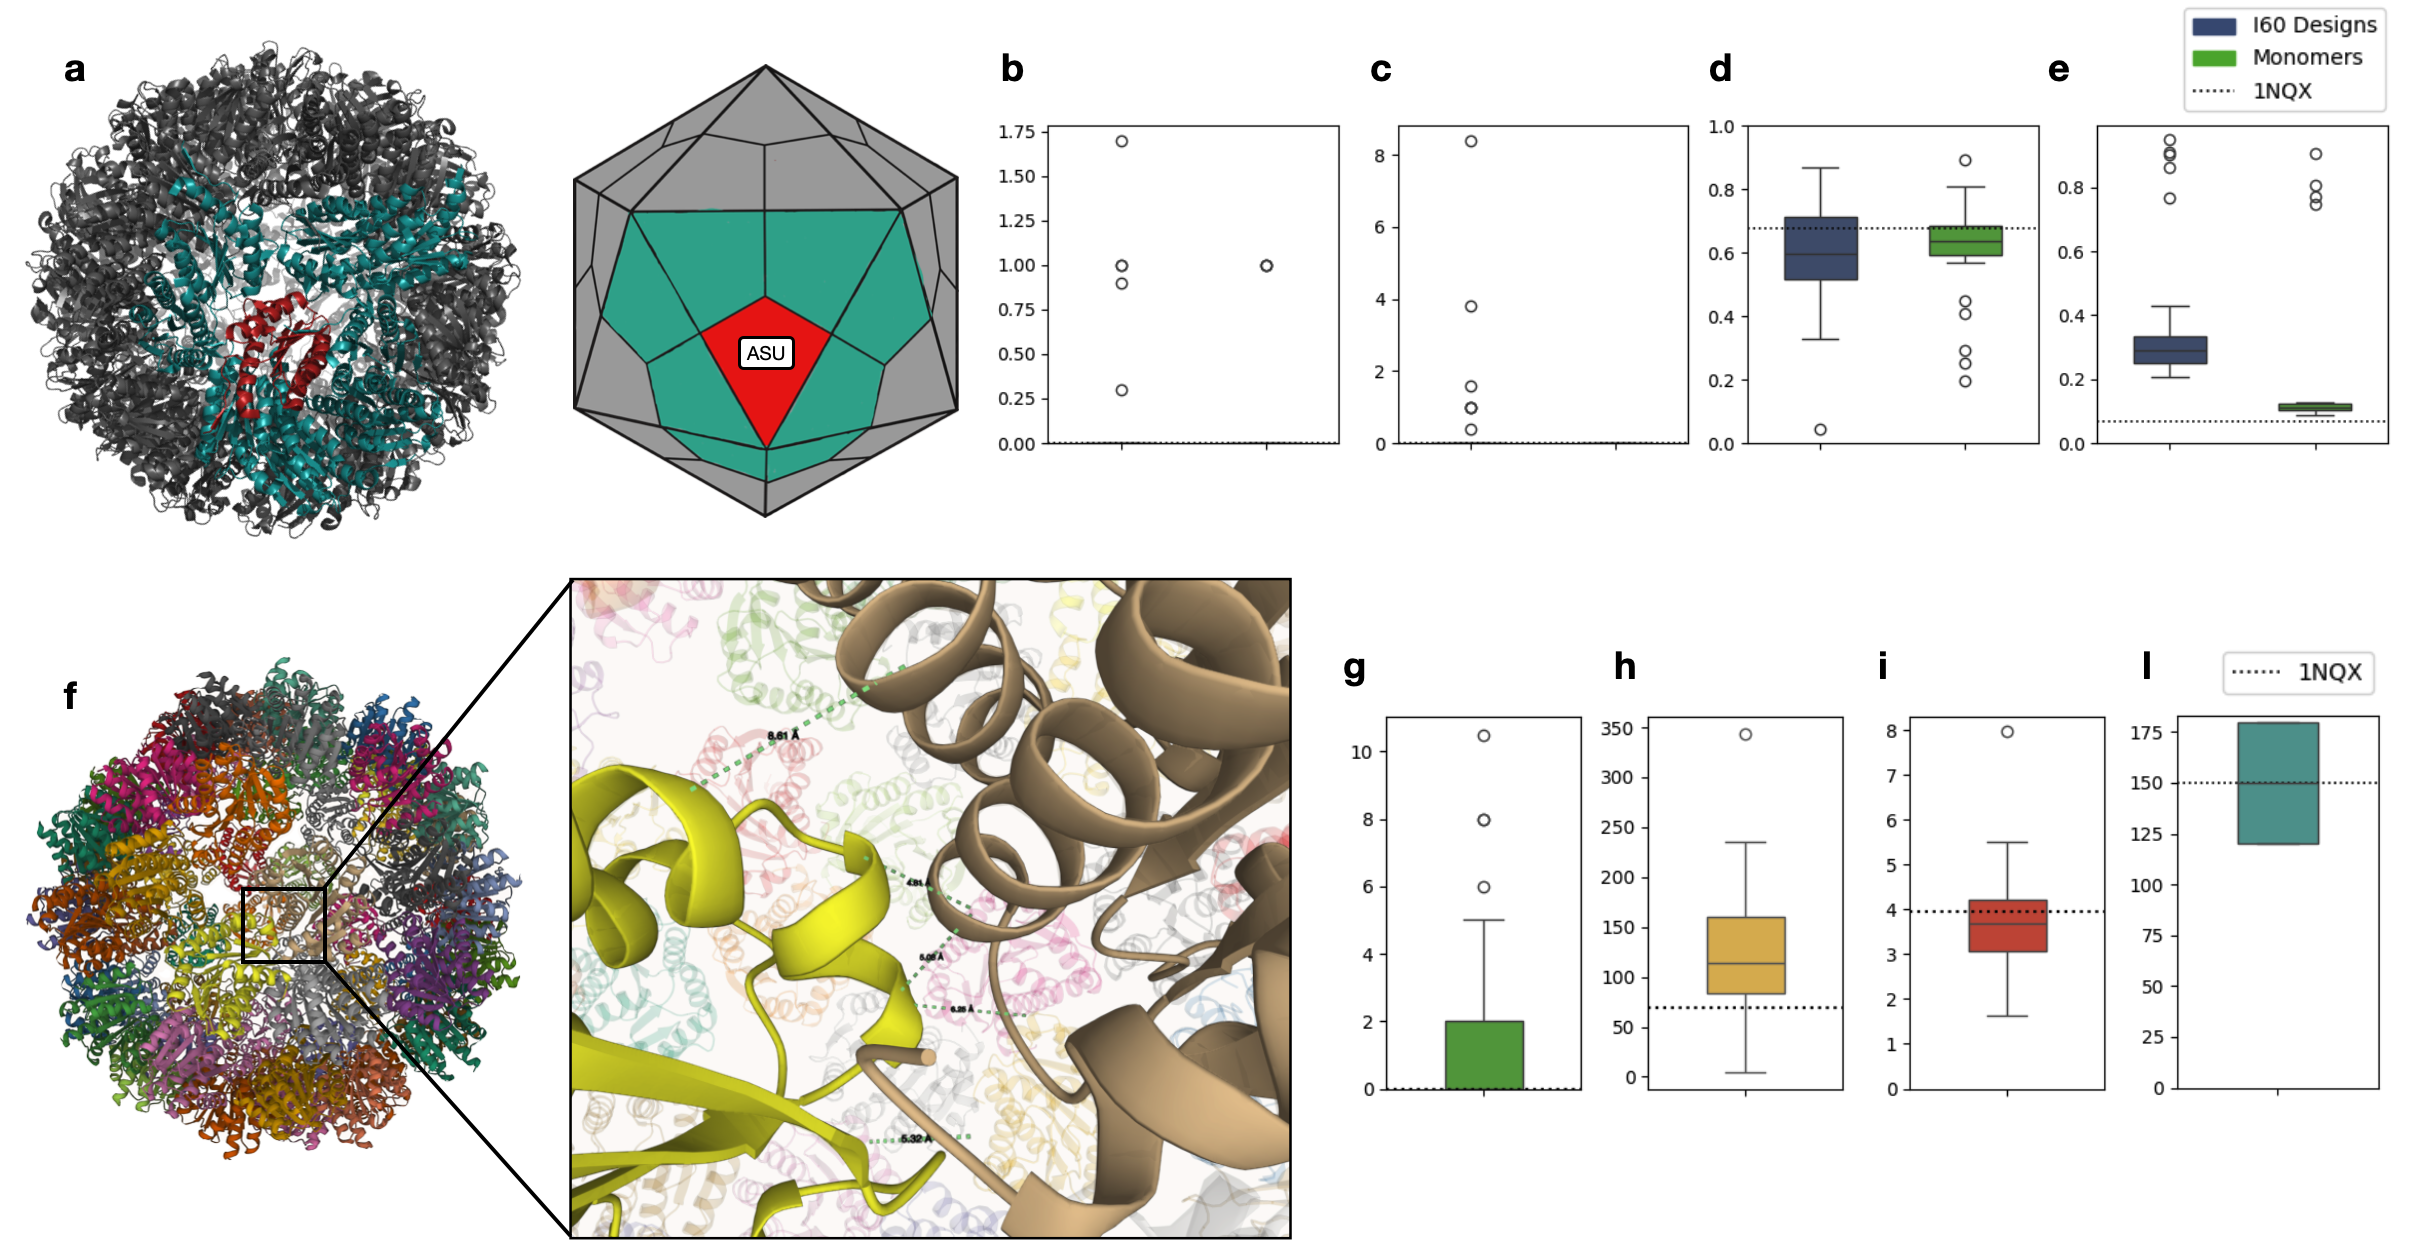
\includegraphics[width=\textwidth]{Figure_2.png}
  \caption{\textbf{Designing icosahedral nanoparticles with Design-CP}
    ($n{=}40$; $60$ chains $\times\,210$ residues $=12{,}600$ residues).
    \textbf{(a)} A single asymmetric subunit (ASU, red) and its neighbouring
    subunits (teal) on the icosahedral shell.
    \textbf{(b--e)} Per-chain backbone-sanity metrics for the icosahedral designs
    (I60) versus $n{=}40$ single-GPU RFD3 monomers, with the lumazine-synthase
    reference (PDB~1NQX, dotted).
    \textbf{(f)} A selected design with a zoom on an inter-ASU interface annotated
    with C$\alpha$--C$\alpha$ distances.
    \textbf{(g--l)} Symmetry-aware interface metrics against the 1NQX baseline.
    Full distributions are reported in Appendix~\ref{app:extended}
    (Figures~\ref{fig:ico-perchain}--\ref{fig:ico-symm}).}
  \label{fig:icosahedral}
\end{figure}

\paragraph{Per-chain backbone quality broadly matches the original RFD3.}
On the backbone-sanity indicators (Figure~\ref{fig:icosahedral}b--e), the two
populations have broadly similar distributions: the average number of chain breaks
per chain and the average count of backbone heavy-atom clashes per chain both have
medians at zero. The ASUs extracted from the nanoparticles designed with Design-CP
show, however, more outliers than the designed monomers, especially for the number
of backbone clashes. The fraction of residues assigned to a helix or
$\beta$-strand element is closely matched between them and to the 1NQX reference
(medians of $\approx 0.60$ for the icosahedral ASUs against $\approx 0.65$ for
monomers, and $\approx 0.68$ for 1NQX). A more notable gap appears in the maximum
per-chain deviation of consecutive C$\alpha$--C$\alpha$ bond lengths from the
canonical \SI{3.8}{\angstrom} value: monomers have a distribution concentrated
around $\approx \SI{0.15}{\angstrom}$, whereas the icosahedral ASUs show a broader
bulk around $\approx \SI{0.30}{\angstrom}$. We partially attribute these
differences to the geometric strain of having to remain self-consistent with
$59$ symmetry mates and all of the inter-subunit interfaces they form, inside a
$12{,}600$-residue joint context, rather than to a degradation introduced by the
context-parallel sampler itself. The icosahedral design problem is strictly harder
per chain than designing monomers of the same length.

\paragraph{Symmetric interfaces track a functional natural assembly.}
Symmetry-aware metrics (Figure~\ref{fig:icosahedral}g--l) generally follow the
1NQX baseline, but not every sample produces a sterically clean assembly. The
number of inter-subunit clashes within the ASU's neighbourhood is non-zero for a
substantial fraction of designs, despite the mean being around zero.
Concordantly, the minimum C$\alpha$--C$\alpha$ distance between distinct chains is
centred near the 1NQX reference at $\approx \SI{4}{\angstrom}$, but the lower tail
of the distribution descends toward and below the \SI{3.5}{\angstrom}
steric-overlap threshold, indicating that a fraction of designs realise inter-chain
contacts inside the steric-overlap regime. The average number of
C$\alpha$--C$\alpha$ contacts per inter-subunit interface centres around
$\approx 125$, slightly above 1NQX rather than collapsing toward zero, and the
number of interfaces making contact resembles that of 1NQX. Combined with the
local visual evidence from the selected sample in
Figure~\ref{fig:icosahedral}f, where ASU--ASU contacts settle into well-formed
packing geometries with C$\alpha$--C$\alpha$ distances in the expected
\SIrange{4}{10}{\angstrom} band, this indicates that the symmetrised denoising
trajectory can recover physically reasonable inter-subunit interfaces rather than
independently designing non-interacting chains.

Together, these results show that Design-CP scales RFD3 sampling to large
icosahedral assemblies without retraining or fine-tuning, broadly preserving
per-chain backbone quality on par with vanilla RFD3 monomers and producing
symmetry-consistent interfaces comparable to a functional natural icosahedral
particle. Full metric distributions are reported in
Appendix~\ref{app:extended}.


\begin{table*}[!t]
  \centering
  \small
  \caption{\textbf{Scaling of Design-CP under icosahedral symmetry.} For each GPU count $P$,
   we report the maximum ASU length before out-of-memory and the wall-clock inference time 
   \emph{at that maximum ASU length}, for the 1D and 2D sharding schemes. 
   \emph{Capacity ratio} is defined as $L_{\max}^{\mathrm{2D}}/L_{\max}^{\mathrm{1D}}$ 
   and \emph{speedup} as $t_{\mathrm{1D}}/t_{\mathrm{2D}}$, so that values greater than 
   unity indicate that the 2D scheme outperforms the 1D scheme. All measurements use HG200 
   GPUs (95\,GB each); a dash denotes a configuration that cannot be measured.}
  \label{tab:scaling}
  \begin{tabular}{rcccccc}
    \toprule
    & \multicolumn{3}{c}{\textbf{Max ASU length before OOM} (residues)} & \multicolumn{3}{c}{\textbf{Wall-clock time at max ASU} (s)} \\
    \cmidrule(lr){2-4} \cmidrule(lr){5-7}
    $P$ & \textbf{1D} & \textbf{2D} & \textbf{Capacity ratio} & \textbf{1D} & \textbf{2D} & \textbf{Speedup} \\
    \midrule
    1  & 58  & 58  & $1.00\times$ & 1023 & 1025 & $1.00\times$ \\
    2  & 102 & --  & --           & 2340 & --   & --           \\
    3  & 120 & --  & --           & 2943 & --   & --           \\
    4  & 141 & 137 & $0.97\times$ & 4321 & 2230 & $1.94\times$ \\
    5  & 160 & --  & --           & 3845 & --   & --           \\
    6  & 173 & --  & --           & 3662 & --   & --           \\
    7  & 186 & --  & --           & 4802 & --   & --           \\
    8  & 196 & --  & --           & 4689 & --   & --           \\
    9  & 201 & 201 & $1.00\times$ & 7247 & 3253 & $2.23\times$ \\
    16 & 219 & 237 & $1.08\times$ & 7030 & 3785 & $1.86\times$ \\
    \bottomrule
  \end{tabular}
\end{table*}

\section{Scaling: max ASU size and inference time vs. number of GPUs}
\label{sec:results-scaling}

To validate the extent of applicability of our proposed CP techniques, 
we performed a scaling analysis on the task of designing proteins with icosahedral
point-group symmetry. Specifically, we target the icosahedral symmetry and sweep the 
amino-acid length of the asymmetric subunit (ASU) until inference runs out of memory (OOM)
for a fixed number of GPUs $P$. \Cref{tab:scaling} shows these values and the inference 
time for that specific run right before reaching OOM error. Unless explicitly mentioned,
all experiments in this subsection use HG200 GPUs with 95\,GB memory and a batch size of
one.

\subsection{Maximum ASU size.}
With either sharding scheme, the dominant quadratic pair tracks are distributed across 
the device mesh, so the memory ceiling is set primarily by the \emph{aggregate} available 
memory rather than by a single-device limit.  We believe this is the reason why we observe 
this value of max ASU length before OOM to be similar, independently of the sharding scheme
used.  Empirically, the maximum feasible ASU length increases with $P$ with the expected 
square-root trend predicted in \Cref{sec:cp-1d,sec:cp-2d}: as $P$ grows linearly while all the 
GPUs are maximally used, each device stores a quadratically smaller proportion of the 
growing pair tensors. 

\subsection{Inference time.}
While the two schemes reach comparable memory ceilings at a given $P$, their wall-clock 
scaling differs. The 1D scheme performs a single \textsc{AllGather} of the single-track 
activations after each attention block (\cref{sec:cp-1d}), which introduces a latency cost 
that grows with cluster size and impacts runtime. The 2D scheme replaces global gathers 
with $\sqrt{P}$-step ring communication over smaller shards and overlaps these shifts with 
local computation (\cref{sec:cp-2d}), yielding better time scaling in practice. This effect is 
reflected in \Cref{tab:scaling}, where 2D CP achieves lower per-step inference time at the 
same $P$, often finishing inference in around half the time with respect to the 1D inference.

% Ensure Table~\ref{tab:scaling} is placed before the next two-column figure.


\subsection{Designing octahedral nanoparticles on small GPUs}
\label{sec:results-democratization}

Octahedral protein cages are a promising but underexplored therapeutic scaffold class: their
rigid, multivalent geometry is suited to higher-order receptor engagement, and their 
interior volume can encapsulate biologic cargoes. Despite this potential, only a few 
\emph{de novo} octahedral cages have been characterised in therapy-relevant cell-based 
functional assays~\parencite{divine_designed_2021,yang_computational_2024}, and as noted in 
\cref{ch:current-memory-reduction-methods}, the memory cost of jointly sampling such large symmetric assemblies 
has been a practical barrier to broadening this design space.

To test whether Design-CP lifts this barrier on commodity hardware, we repeated the 
scaling protocol of \cref{sec:results-scaling} for octahedral targets, this time using a 
small cluster of workstation-grade NVIDIA RTX~A4000 GPUs ($16$\,GB per device,
${\sim}6\times$ less per-device memory than the HG200 GPUs used so far) and we report the 
results in \cref{app:O24_scaling_and_metrics}. In practice, the 2D sharding scheme allowed 
us to sample full octahedral assemblies up to $178$ residues per chain (with $24$ chains, 
this means modelling $4{,}272$ residues total) on $16$ A4000 GPUs 
(\cref{fig:octahedral}a), a per-chain size comparable to existing \emph{de novo} 
octahedral nanoparticles~\parencite{king_computational_2012}; we then evaluated $n=12$ such 
designs against the same families of \emph{in silico} metrics used for the icosahedral 
targets in \cref{sec:icosahedral}. Additional metrics and a discussion of the scaling 
sweep on this hardware are deferred to Appendix~\ref{app:O24_scaling_and_metrics}.

\subsection{Backbone sanity tracks the icosahedral baseline.} 
The backbone quality indicators (\cref{fig:octahedral}b--e) are healthy and
consistent with the icosahedral designs population: the per-chain count of chain breaks 
concentrates at zero with a single outlier at $2$, the count of backbone heavy-atom clashes 
is essentially zero across all designs (one outlier near $70$), the fraction of residues 
assigned to a helix or strand element sits at a median of $\approx 0.65$, and the maximum 
per-chain deviation of consecutive C$\alpha$--C$\alpha$ bond lengths from the canonical 
$3.8$\,\AA{} value clusters tightly around $\approx 0.3$\,\AA{}, well below the 
$0.75$\,\AA{} chain-break threshold. This last distribution is in fact noticeably tighter 
than for the icosahedral chains, and might suggest that the lower oligomeric state 
($24$ vs.\ $60$ subunits) imposes less geometric strain per chain.

\subsection{Symmetric interfaces are well-formed.} 
The two main symmetry-interface metrics shown in \cref{fig:octahedral}f--g are 
likewise healthy. The minimum C$\alpha$--C$\alpha$ distance between distinct chains sits 
in the $\approx 4$--$10$\,\AA{} band, consistent with proper inter-subunit packing without 
steric overlap, and the average number of C$\alpha$--C$\alpha$ contacts per inter-subunit 
interface centres around $\approx 30$ with a positive tail beyond $60$. An example of 
octahedral design is provided in \cref{fig:octahedral}a, where the chains organise 
into a closed, octahedrally symmetric cage. This confirms that the symmetrised trajectory 
realises the intended point-group geometry with favourable \emph{in silico} metrics on commodity 
GPUs.\\

Overall, these results indicate that large-assembly protein design can be made feasible 
on modest, widely available GPU hardware, lowering the barrier to entry for groups without 
access to large-memory accelerators.



\begin{figure}[t]
  \centering
  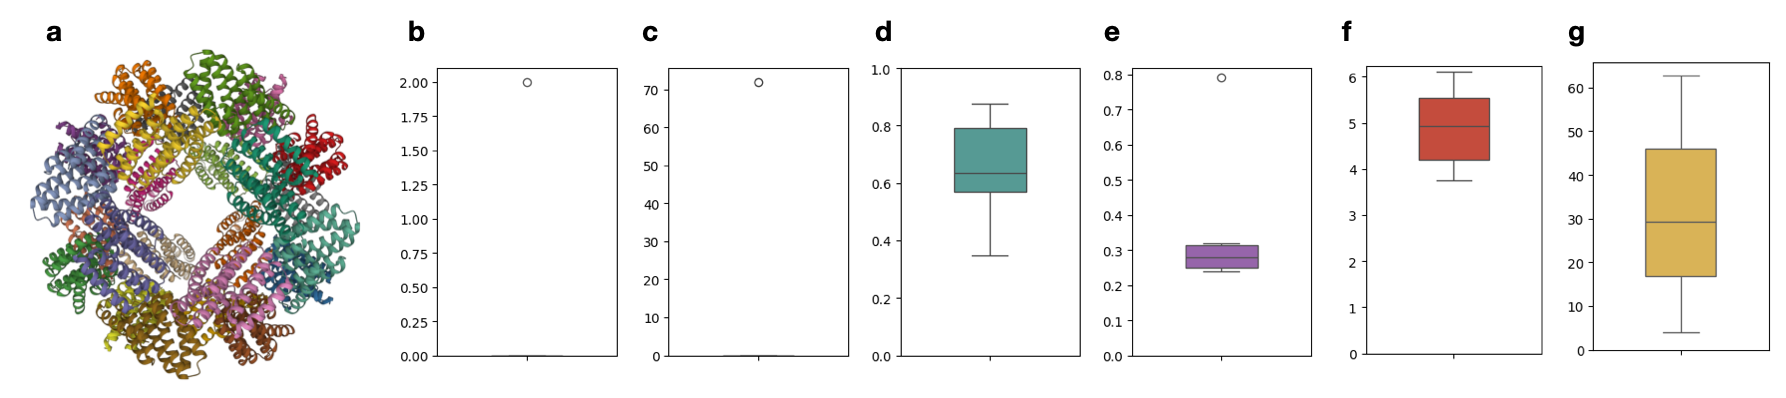
\includegraphics[width=\textwidth]{Octahedral_figure_main_text.png}
  \caption{\textbf{Designing octahedral nanoparticles on workstation-grade GPUs.}
   \textbf{a}, A representative Design-CP octahedral assembly with $176$ residues per 
   chain ($24$ chains, $4{,}224$ residues total) generated on $16$ NVIDIA RTX~A4000 GPUs 
   ($16$\,GB per device). \textbf{b--e}, Backbone-sanity metrics over $n=12$ such designs: 
   \textbf{b} chain breaks, \textbf{c} backbone clashes, \textbf{d} non-loop fraction, 
   \textbf{e} max CA deviation. \textbf{f--g}, Symmetry-interface metrics: \textbf{f} 
   minimum inter-chain distance, \textbf{g} mean contacts per interface. Metric definitions
    in Appendix~\ref{app:designability}; the remaining secondary-structure and contact 
    metrics are reported in Appendix~\ref{app:O24_scaling_and_metrics}.}
  \label{fig:octahedral}
\end{figure}


\section{Discussion}
\label{sec:discussion}

We introduced \emph{Design-CP}, two context-parallel inference strategies for RFDiffusion~3 
that shard the quadratic token- and atom-pair representations across multiple GPUs while 
preserving the model's architecture and weights. We characterised the memory ceilings and 
strong-scaling behaviour of a lightweight 1D row-sharding scheme and a 2D grid scheme 
(which requires a perfect-square GPU count $P$ to form a $\sqrt{P}\times\sqrt{P}$ mesh), 
and found that 2D sharding achieves better wall-clock scaling in practice by overlapping 
ring communication with computation.

Beyond RFD3, the underlying approach is model-agnostic: any protein design model whose 
inference is dominated by self-attention and other $\mathcal{O}(n^2)$ pairwise activations 
can, in principle, adopt the same sharding patterns. This suggests that context parallelism
is broadly applicable across modern design pipelines, which largely build on 
Transformer-style attention mechanisms with pari-bias.

We further showed that strong point-group symmetry constraints can make CP usable 
\emph{out of the box} for end-to-end all-atom design of large protein nanoparticles 
without retraining or fine-tuning. Prior work on context-parallelism for structure 
prediction (e.g., Fold-CP, \cite{lin_fold-cp_2026}) indicates that scaling inference to 
very large complexes can be limited by out-of-distribution generalisation once inputs exceed 
the model's native training regime. Our results refine this picture: for highly symmetric 
assemblies, symmetrised sampling collapses the effective degrees of freedom to a single ASU 
while still modelling the correct inter-subunit geometry, enabling CP to scale to full 
icosahedral and octahedral assemblies while preserving promising \emph{in silico} backbone-sanity 
and symmetry-interface metrics (\cref{sec:icosahedral,sec:results-democratization}). We 
also demonstrated that the same approach enables \emph{de novo}
design of octahedral nanoparticles on a small cluster of workstation-grade GPUs, indicating 
a practical path towards democratising large-assembly protein design.

A key limitation is that pushing beyond the native training crop can still introduce 
distribution shift and degrade outputs for highly asymmetric targets. Future work could 
therefore explore training or fine-tuning design models with longer contexts and/or explicit 
context-parallelism in the training loop. This is now not a priority for this project, as our
immediate goal is to design large symmetric assemblies for vaccine applications, but it is a 
natural next step for the broader design community.

% as well as experimental validation of the d
% esigned assemblies to assess how \emph{in silico} quality metrics translate to expression, 
% stability, and correct self-assembly \emph{in vitro}.

%==============================================================================
% Chapter 5 -- Future work
%==============================================================================
\chapter{Future work}
\label{ch:future-work}

% -----------------------------------------------------------------------------
% The "expanding funnel": start from a very concrete immediate next step and
% widen to a multi-year research vision, closing with a Gantt chart. Edit the
% pgfgantt block at the end to match your real milestones and dates.
% -----------------------------------------------------------------------------

Having established that whole symmetric assemblies can be modelled end to end
(Chapters~\ref{ch:methods}--\ref{ch:results}), I now describe the work that
builds on this. Section~\ref{sec:experimental-validation} concerns experimental
validation of the designs, Section~\ref{sec:motif-scaffolding} the extension
from unconditional to symmetric motif scaffolding generation, and
Section~\ref{sec:shape-control} finer control over assembly shape.
Section~\ref{sec:broad-agenda} places these in the context of the wider research
programme, and Section~\ref{sec:gantt} gives the timeline.


\section{From \emph{in silico} metrics to experimental validation}
\label{sec:experimental-validation}

The results of Chapter~\ref{ch:results} are entirely computational. The metrics
of Section~\ref{sec:evaluation} establish that the generated particles are
geometrically sound and that their designed interfaces are comparable to those
of a natural reference particle. They do not establish that a design will
express solubly, fold, or assemble into the intended cage. The usual substitute,
refolding with a structure predictor, is unreliable at this chain count
\parencite{bryant_predicting_2022}, which is why it was avoided here, and
designed assemblies that satisfy computational criteria have been found to be
structurally flexible or oligomorphic when characterised experimentally
\parencite{khmelinskaia_local_2025}. The real value of this proposed method should 
be assessed through experimental validation.

I will spend part of the 2026/27 academic year at the Baker Lab, where the relevant
experimental pipeline is well established. The work there will begin with a
small design campaign: generating a library of assemblies, designing sequences
with ProteinMPNN \parencite{dauparasRobustDeepLearning2022}, filtering on the
metrics of Section~\ref{sec:evaluation}, and expressing the candidates that
pass those filters. Characterisation would proceed in order of increasing cost (as previously done by \cite{haas_novo_2026} and coworkers), beginning
with assays like Immobilized Metal Affinity Chromatograpy (IMAC), Size Exclusion Chromatography (SEC), and chromatography and LC--MS to confirm subunit identity and an elution profile consistent with an assembled particle. These experiments will be followed by negative-stain
electron microscopy to assess morphology, and single-particle cryo-EM for the
most promising candidates. How much of this can be completed within the year
will depend on expression yields and on the number of designs that clear the
early filters.

The campaign would also yield matched computational and experimental outcomes
for assemblies generated end to end rather than docked from pre-computed
building blocks, which is not something currently available for this class of
protiens. Such data would indicate whether the inexpensive geometric filters used
in this report track successful assembly in practice, and would inform the
broader programme described in Section~\ref{sec:broad-agenda}.


\section{From unconditional to conditional generation: symmetric motif scaffolding}
\label{sec:motif-scaffolding}

Design-CP as reported performs \emph{unconditional} generation: it produces a
symmetric particle, but not a particle built around a \emph{specific} antigen. The
natural next step is \emph{conditional} generation, holding many copies of one or more functional
motifs (the antigen, or an epitope we wish to display) fixed while the model
designs a symmetric scaffold that presents them. In the symmetric setting this is
\emph{symmetric motif scaffolding}: the standard motif-scaffolding problem
\parencite{watsonNovoDesignProtein2023,didiFrameworkConditionalDiffusion2024},
recently generalised to atom-level motifs without known sequence indices
\parencite{ahern_atom_2025}, composed with the
point-group machinery of Section~\ref{sec:rfd3-prelim}, so that a motif placed in
one ASU (or at symmetric interface between some ASUs) is presented at every symmetry-equivalent 
position on the particle. This work will be
carried out in collaboration with the Baker Lab during a visit there in the next
academic year (2026/27), giving direct access to their design and experimental
pipelines for validating conditionally designed immunogens.

\section{Greater control over the shape of generated assemblies}
\label{sec:shape-control}


Particle radius is already controllable within the framework of
Chapter~\ref{ch:methods}, but there are other geometric features that a protein designer might want to design for. Two are of
particular interest. First, the currently generated assemblies show pores at some interfaces that arise as a by-product of the design rather than as a specified feature. Second, natural capsid subunits frequently possess extended arms that interdigitate with neighbouring subunits, a feature with clear structural
consequences: the N-terminal arm forms the $\beta$-annulus underlying
quasi-equivalence in $T{=}3$ plant viruses \parencite{harrison_protein_2017}, and
C-terminal arm exchange allows papillomavirus and polyomavirus pentamers to
occupy hexavalent positions in a $T{=}7$ lattice
\parencite{liddingtonStructureSimianVirus1991}. Since the training distribution is dominated
by globular monomers, such subunits fall outside what the model readily
produces.

Both features are geometric, which suggests shape conditioning as a route to
controlling them. Building on existing spatial conditioning methods
\parencite{ingrahamIlluminatingProteinSpace2023,stark_protcomposer_2025,faltings_proxelgen_2025,raghu_multiscale_2025,li_robust_2026},
I plan to let the designer specify a target envelope that the model must
respect, which would make pore size and position explicit design variables and
allow non-globular subunits to be requested directly.


\section{A broader agenda: designing large symmetric protein assemblies}
\label{sec:broad-agenda}

More broadly, and over the remainder of the DPhil, I will continue to study the
design of large, and often symmetric, protein assemblies as a subject in its own
right. Doing this well requires understanding, and learning to design for, the
factors that govern whether subunits actually come together: specific
protein--protein interactions at the designed interfaces and the
thermodynamics of self-assembly, the functional and physicochemical drivers of
symmetric oligomerisation \parencite{goodsell_structural_2000} and the multistep,
ordered assembly pathways documented for natural complexes
\parencite{marsh_structure_2015}, and phenomena such as the structural
flexibility and oligomorphism observed in designed assemblies
\parencite{khmelinskaia_local_2025}.
The space of targets is correspondingly wide, from vaccine scaffolds to
mechanically coupled molecular machines \parencite{courbet_computational_2022} and
allosterically switchable assemblies \parencite{pillai_novo_2024}.

\section{Timeline and milestones}
\label{sec:gantt}

Figure~\ref{fig:gantt} summarises the plan on a single timeline: the work
packages of Sections~\ref{sec:motif-scaffolding}--\ref{sec:broad-agenda}, the
papers and conferences they are aimed at, and the two formal milestones of the
DPhil.

\clearpage % put the Gantt chart on its own page so it can't overlap the text above
\begin{figure}[H]
  \centering
  \hspace*{-1.2cm}% shift the chart left (tweak as needed)
  \begin{ganttchart}[
      hgrid, vgrid,
      x unit=1.45cm,
      y unit title=0.6cm,
      y unit chart=0.75cm,
      title height=1,
      title/.append style={fill=oxfordblue!12},
      title label font=\footnotesize\bfseries,
      bar/.append style={fill=oxfordblue!75, rounded corners=1.5pt},
      bar height=0.55,
      bar label font=\footnotesize,
      bar label node/.append style={text width=5.2cm, align=right},
      group/.append style={fill=oxfordblue},
      group height=0.55,
      group label font=\footnotesize\bfseries,
      group label node/.append style={text width=5.2cm, align=right},
      milestone/.append style={fill=orange!85},
      milestone height=0.55,
      milestone label font=\footnotesize\itshape,
      milestone label node/.append style={text width=5.2cm, align=right},
      group right shift=0,
      group left shift=0,
    ]{1}{8}
    % --- title rows: years and quarters (TODO: adjust to your real timeline) ---
    \gantttitle{2026}{2}\gantttitle{2027}{4}\gantttitle{2028}{2} \\
    \gantttitle{Q3}{1}\gantttitle{Q4}{1}%
    \gantttitle{Q1}{1}\gantttitle{Q2}{1}\gantttitle{Q3}{1}\gantttitle{Q4}{1}%
    \gantttitle{Q1}{1}\gantttitle{Q2}{1} \\
    % --- Foundation: whole-assembly modelling ---
    \ganttgroup{Whole-assembly modelling}{1}{5} \\
    \ganttbar{Finalise Design-CP \& submit paper}{1}{2} \\
    \ganttbar{Experimental (in-vitro) validation}{3}{5} \\
    % --- Conditional generation ---
    \ganttgroup{Conditional generation}{3}{8} \\
    \ganttbar{Symmetric motif scaffolding}{3}{6} \\
    \ganttbar{Test on real antigens}{6}{8} \\
    % --- Shape / spatial control ---
    \ganttgroup{Shape \& spatial control}{1}{4} \\
    \ganttbar{Improve spatial/shape\\conditioning}{1}{4} \\
    % --- Broader agenda ---
    \ganttgroup{Large symmetric assemblies}{6}{8} \\
    \ganttbar{PPIs \& thermodynamics\\of assembly}{6}{8} \\
    \ganttbar{Thesis writing}{7}{8} \\
    % --- Papers and conferences ---
    % Each paper bar ends on the submission deadline of the conference it targets:
    % ICML 2027 closes in 2027 Q1, ICLR 2028 in 2027 Q3.
    \ganttgroup{Papers \& conferences}{2}{8} \\
    \ganttbar{Shape-conditioning paper\\(ICML 2027)}{2}{3} \\
    \ganttbar{Symmetric-scaffolding paper\\(ICLR 2028)}{4}{5} \\
    \ganttmilestone{ICML 2027}{4} \\
    \ganttmilestone{ICLR 2028}{7} \\
    % --- Milestones ---
    \ganttmilestone{Transfer of Status}{1} \\
    \ganttmilestone{Confirmation of Status}{5}
  \end{ganttchart}
  \caption{Gantt chart of upcoming milestones and deadlines}
  \label{fig:gantt}
\end{figure}

\clearpage % flush any remaining floats so the Gantt chart stays before references

%------------------------------- References -----------------------------------
\printbibliography[title=References]

%------------------------------- Appendix -------------------------------------
\appendix
%==============================================================================
% Appendix -- Extended in-silico metrics
%==============================================================================
\chapter{Extended in-silico metrics}
\label{app:extended}

This appendix collects the metric definitions, implementation details and full
metric distributions deferred from Chapters~\ref{ch:methods}
and~\ref{ch:results}, together with the octahedral scaling sweep of
Section~\ref{app:O24_scaling_and_metrics}. Each box plot shows the median,
interquartile range and whiskers over the design set, with the
lumazine-synthase reference (PDB~1NQX, dotted) shown where applicable.

\section{Metric definitions}
\label{app:metric-defs}
\label{app:designability}% alias: Figure~\ref{fig:octahedral} cites the metric
                         % definitions under this name.

All quantities are computed directly from the generated all-atom coordinates of
the symmetrised assembly; no external structure-prediction oracle is used. The
metrics fall into two families.

\paragraph{Backbone sanity.}
\emph{Chain breaks} are consecutive C$\alpha$--C$\alpha$ pairs whose bond length
departs from the canonical \SI{3.8}{\angstrom} by more than
$\tau_\text{cb}=\SI{0.75}{\angstrom}$; pairs spanning an intended chain
transition are masked out. The related \emph{maximum C$\alpha$ deviation} is the
worst such departure in a design, reported as a continuous summary rather than a
count. \emph{Backbone clashes} are heavy-atom pairs drawn from residues at least
two apart in sequence and closer than $\tau_\text{clash}=\SI{1.5}{\angstrom}$,
restricted to the backbone atoms $\{\text{N},\text{C}\alpha,\text{C}\}$, which
have no rotameric freedom with which to relieve an overlap; the corresponding
side-chain variant is much noisier and is reported only as a lower bound on
clash density. The \emph{non-loop fraction} is the proportion of residues
assigned to a helix or a strand by the P-SEA annotator
\parencite{labesse_p-sea_1997}, as implemented in Biotite's
\texttt{annotate\_sse}. As secondary filters we also report the radius of
gyration, the separate helix and sheet fractions, the number of
secondary-structure elements from the same annotation, and the per-residue
amino-acid composition, in particular the alanine and glycine content, where a
biased composition often signals a pathological design.

\paragraph{Symmetric-interface sanity.}
These use the full symmetrised complex, excluding any atom belonging to a fixed
or unsymmetrised motif, and all distances are
C$\alpha$--C$\alpha$. Three thresholds apply: a hard inter-subunit clash distance
of \SI{3.5}{\angstrom}, a contact band of \SIrange{4.0}{10.0}{\angstrom}, and a
proximity cutoff of \SI{15.0}{\angstrom} beyond which two subunits count as
non-interacting. \emph{ASU clashes} count inter-subunit pairs below the clash
distance, normalised by the number of subunits so that the figure is comparable
across point groups of different order. \emph{Mean contacts per interface}
counts, for every pair of subunits within the proximity cutoff, the pairs falling
inside the contact band, averaged over those interfaces. \emph{Minimum
inter-chain distance} is the smallest such distance anywhere in the complex:
values below roughly \SI{3.5}{\angstrom} indicate steric overlap, while values
well above \SI{6}{\angstrom} indicate that the subunits never meet, which for a
closed particle is itself a failure. The \emph{total interface contacts} is the
unnormalised sum of the contact counts over all interfaces, while the
\emph{number of interfaces with contacts} and the \emph{minimum contacts per
interface} together flag assemblies in which one interface is effectively absent
even though the mean is healthy. Finally, the \emph{minimum intra-ASU distance}
is the smallest C$\alpha$--C$\alpha$ distance \emph{within} a single subunit,
which catches intra-subunit overlap that the inter-subunit clash count cannot
see.

\section{Implementation notes}
\label{app:implementation}

\paragraph{Per-step symmetrisation.}
At each denoising step within the symmetrised portion of the trajectory:
(i)~Gaussian noise is added to the current coordinates and the noised structure is
itself symmetrised, so the network receives an exactly symmetric input
$\mathbf{X}^{(t)}$; (ii)~the network predicts clean coordinates
$\hat{\mathbf{X}}_0$ for all chains, which need not be exactly symmetric;
(iii)~the prediction is centred, the ASU slice is extracted and centred, and every
subunit (including the ASU itself) is rebuilt as
$R_g\,\hat{\mathbf{X}}_{0,\text{ASU}} + \lambda\,\mathbf{t}_g$, where
$\{(R_g,\mathbf{t}_g)\}_{g=1}^{G}$ are the rigid-body transforms of the chosen
point group and $\lambda$ is a scale factor that adapts the inter-subunit distance
to the current prediction; in the second half of the trajectory, a short
Lennard-Jones-based rigid-body optimisation of the ASU against its symmetry copies
is applied before this step to reduce inter-subunit clashes; (iv)~this symmetrised
prediction is used in the EDM update \parencite{karras_elucidating_2022}. For the
final $10\%$ of steps, no symmetry is enforced, allowing the model to relax any
residual strain at the inter-subunit interfaces before output.

\paragraph{Chunk distribution.}
Device $p$ receives $I_p$ rows as in Equation~\eqref{eq:row-stripe}, starting at
$p\lfloor I/P\rfloor + \min(p,\, I \bmod P)$. Uneven chunks are handled by padding
each local tensor to the per-rank maximum before the collective and trimming the
concatenated result back to $I$.

\paragraph{Communication volume.}
The dominant cost of the 1D scheme is the eighteen \texttt{ALLGATHER} calls on the
token track issued by the diffusion transformer per recycling iteration, with two
recycling iterations per denoising step. Each rank's message is sized by the token
count and channel width and is therefore independent of $P$, so the term that
grows with the device count is collective latency rather than payload.

\paragraph{Determinism.}
The two schemes reach determinism by different routes. In the 1D scheme the
atom-to-token pooling uses an index reduction whose floating-point accumulation
order depends on device scheduling, so ranks disagree slightly; because those
pooled features become the keys and values of the following cross-attention, the
discrepancy is amplified and breaks the requirement that all ranks hold identical
keys and values. A single broadcast of the pooled features immediately after the
reduction restores the invariant. The 2D scheme implements the same pooling as a
distributed scatter-reduce collective, which is deterministic by construction and
needs no broadcast. The two schemes also keep the sampling loop itself consistent
by different routes: the 1D scheme broadcasts the sampled noise and the denoised
prediction from rank~$0$ at each step boundary, whereas the 2D scheme draws the
full-shape noise tensor from per-rank generators held in lockstep and shards it
afterwards, so that no broadcast is required. Either way, a given seed produces
the same trajectory under either scheme.

\paragraph{Distributed nearest neighbours.}
The sparse atom attention needs the $k$ nearest neighbours of every query atom,
which a naive implementation obtains from an $L\times L$ distance matrix, the very
object that cannot be afforded at these scales. Instead, each device computes
distances between its local atom rows and those resident on its column partner,
in chunks, so that even the per-quadrant block is never held in full; a ring
reduction then merges partial top-$k$ candidates around the column axis over
$\sqrt{P}$ steps. After the final step each device holds the global top-$k$
indices for its own query atoms, and no $L\times L$ tensor is materialised on any
device at any point.

\clearpage
\section{Icosahedral designs}
\label{app:ico}

The comparison in Figure~\ref{fig:icosahedral}b--e covers four panels: chain
breaks, backbone clashes, non-loop fraction and maximum C$\alpha$ deviation.
Figure~\ref{fig:ico-perchain} shows the full eight-panel version, adding helix
fraction, sheet fraction, glycine content and the average number of
secondary-structure elements per chain.

\paragraph{Caveat on problem difficulty.}
The two design problems are not of equal difficulty, and the comparison should be
read with this asymmetry in mind. Each icosahedral chain is denoised inside a
$12{,}600$-residue joint context, where its trajectory must remain
self-consistent with the simultaneously denoised trajectories of $59$ symmetry
mates and with all the inter-chain interfaces they form, whereas the monomer
problem is a single $210$-residue chain comfortably inside RFD3's native
$384$-token training crop. The icosahedral problem is therefore strictly harder
per chain.

\paragraph{Helix and sheet fraction.}
The most prominent qualitative gap in Figure~\ref{fig:ico-perchain} appears in
secondary-structure composition. Vanilla RFD3 monomers reproduce a helix/sheet
balance close to that of the 1NQX reference: the helix fraction concentrates
around a median of $\approx 0.47$ with a tight bulk against the 1NQX value of
$0.47$, and the sheet fraction sits at a median of $\approx 0.18$ with a
comparable spread, against $0.20$ for 1NQX. The Design-CP icosahedral designs, in
contrast, are strongly $\beta$-biased: the helix fraction collapses near zero on
the bulk of chains, with a few upper outliers, and the sheet fraction shifts
upwards to a median of $\approx 0.5$ with a noticeably broader distribution.

\paragraph{Number of secondary-structure elements.}
Consistent with the helix/sheet shift, the average number of secondary-structure
elements per chain rises from $\approx 13$ in the monomers to $\approx 16$ in the
icosahedral designs, with the icosahedral distribution carrying a heavier upper
tail; both populations include outliers, but only the icosahedral set reaches the
upper twenties. At fixed chain length a higher element count mechanically implies
shorter average elements, which is again consistent with the icosahedral chains
preferring multiple short $\beta$-strands over a small number of long helices. We
treat this as supportive evidence for the helix/sheet shift rather than an
independent observation, and note that the metric is sensitive to the P-SEA
assignment thresholds \parencite{labesse_p-sea_1997}.

\paragraph{Amino-acid composition.}
On amino-acid composition the two populations are closer to each other than on
secondary structure. Alanine content is similar across both sets, with broadly
overlapping distributions and medians of the same order, and is, as is typical
for RFD3 \parencite{butcher_novo_2025}, slightly inflated relative to 1NQX in
both cases; we do not read a meaningful difference between Design-CP ASUs and
vanilla monomers on this axis. Glycine content, in contrast, is appreciably
broader in the icosahedral designs ($\approx 0.10$--$0.25$, with sporadic high
outliers) than in the monomers ($\approx 0.05$--$0.10$, very tightly
concentrated), although the medians remain of the same order and within the
typical range for natural proteins. The widened glycine spread is qualitatively
consistent at the population level with the broader maximum
C$\alpha$--C$\alpha$ deviation of Figure~\ref{fig:icosahedral}e, chains under
greater inter-subunit strain relying more on backbone-flexible residues, but we
flag this as a tentative association rather than a causal claim, since we have
not tested whether the same chains drive both effects.

\begin{figure}[h]
  \centering
  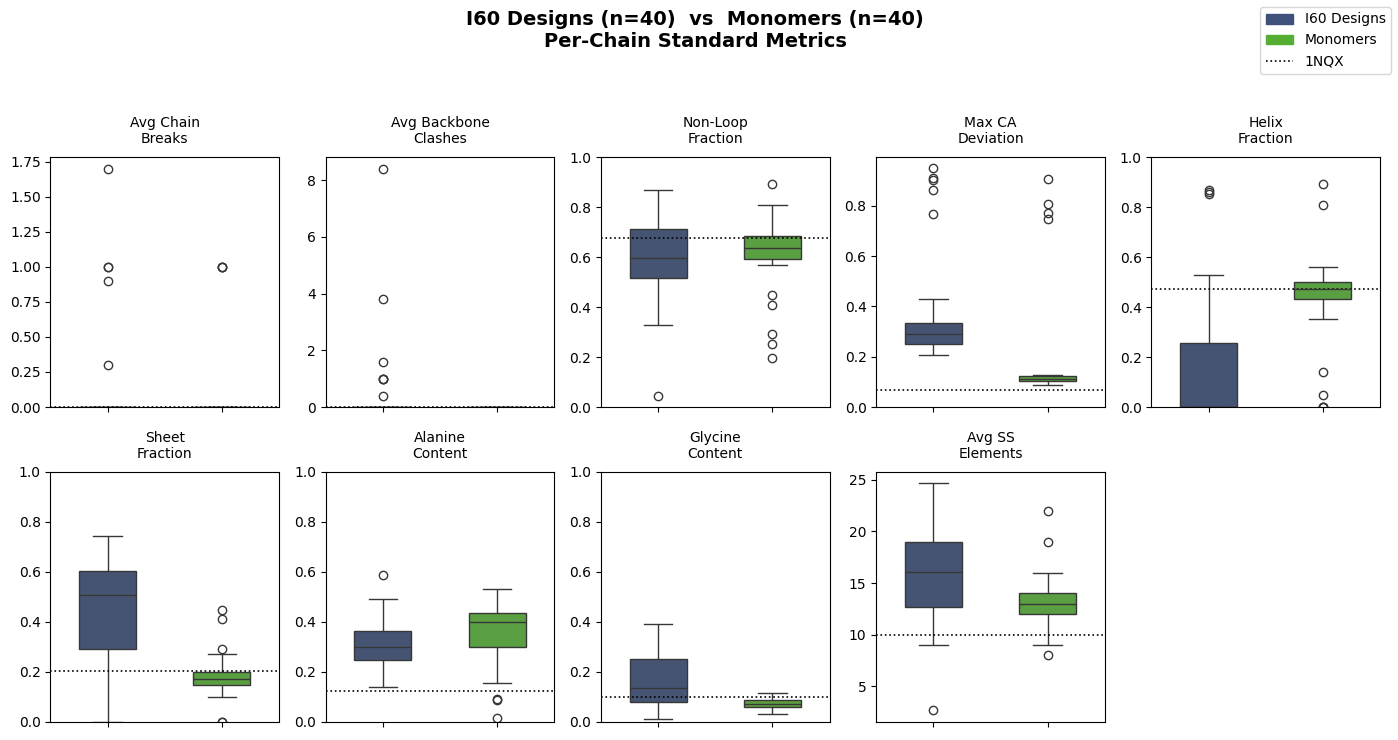
\includegraphics[width=\textwidth]{RFD3-vs-DesignCP.png}
  \caption{\textbf{Per-chain comparison of Design-CP icosahedral designs against
    vanilla RFD3 monomers (full eight panels).} Backbone-sanity and composition
    metrics computed chain by chain on $n{=}40$ Design-CP icosahedral assemblies
    ($60$ chains $\times\,210$ residues) and $n{=}40$ vanilla single-GPU RFD3
    monomers of length $210$, with the lumazine-synthase reference (PDB~1NQX)
    dotted in each panel. The first four panels reproduce
    Figure~\ref{fig:icosahedral}\textbf{b--e}; the additional four (helix
    fraction, sheet fraction, glycine content, average number of
    secondary-structure elements) show the secondary-structure shift discussed
    above.}
  \label{fig:ico-perchain}
\end{figure}

\begin{figure}[h]
  \centering
  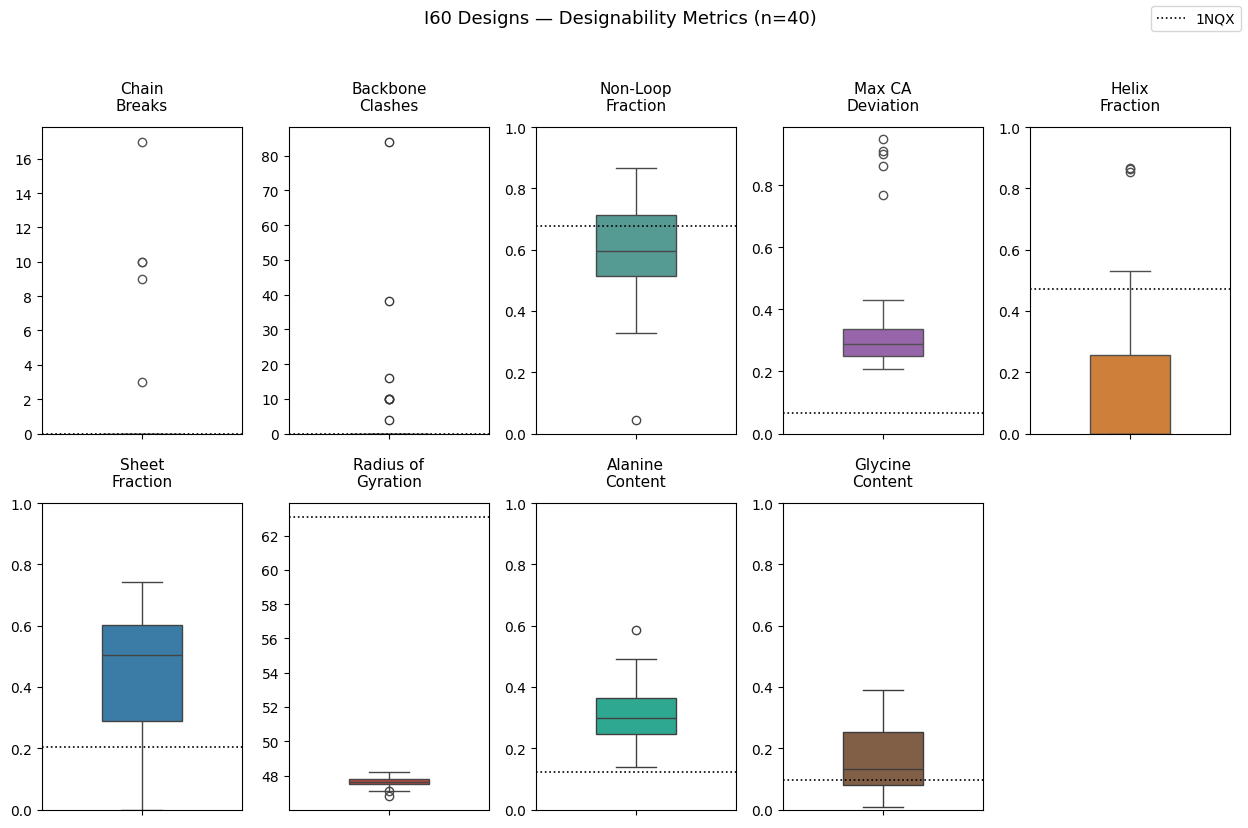
\includegraphics[width=\textwidth]{Icosahedral_designability_metric_ASU.png}
  \caption{Full designability (backbone-sanity) distributions for the icosahedral
    I60 designs ($n{=}40$), including radius of gyration.}
  \label{fig:ico-des}
\end{figure}

\begin{figure}[h]
  \centering
  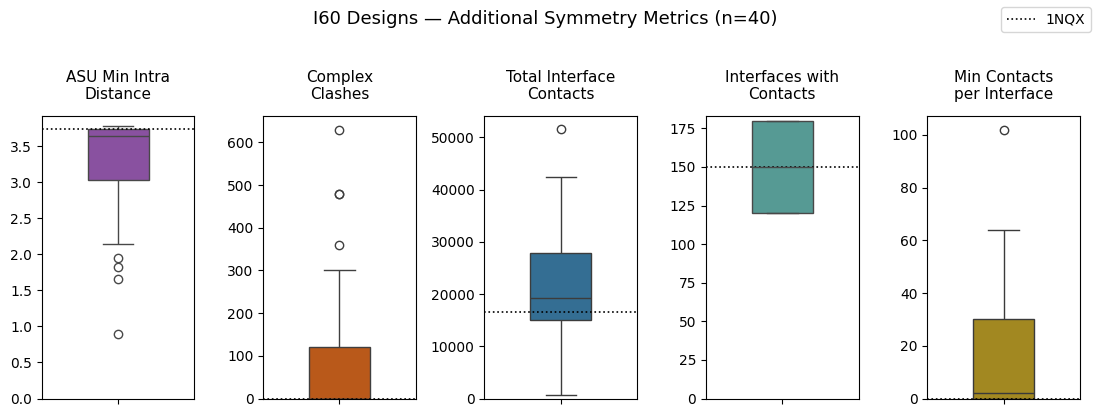
\includegraphics[width=\textwidth]{Icosahedral_symmetry_metrics_extra.png}
  \caption{Additional symmetry-aware interface metrics for the icosahedral I60
    designs ($n{=}40$), extending Figure~\ref{fig:icosahedral}\textbf{g--l}.}
  \label{fig:ico-symm}
\end{figure}

\clearpage
\section{Octahedral designs on workstation-grade GPUs}
\label{app:O24_scaling_and_metrics}
\label{app:oct}

This section collects the material deferred from
Section~\ref{sec:results-democratization}: the scaling sweep for octahedral
targets on workstation-grade hardware, and the metric distributions not shown in
the main-text figure.

\subsection*{Maximum assembly size on RTX~A4000 GPUs}

The sweep follows the protocol of Section~\ref{sec:results-scaling}: at a fixed
device count we increase the ASU length until inference runs out of memory, and
record the last feasible length. The only difference is the hardware. Each
RTX~A4000 provides $16$\,GB of device memory against the
$95$\,GB of a GH200, roughly a sixfold reduction per device, so even
the aggregate memory of the whole A4000 cluster is below that of a single GH200.
Because octahedral symmetry has order $24$, a given ASU length here corresponds
to an assembly of $24$ chains rather than the $60$ of the icosahedral case, and
the token and atom counts entering the quadratic pair tracks scale accordingly.

On $16$ A4000s the 2D scheme reached a ceiling of $178$ residues per chain, that
is $4{,}272$ residues over the full assembly, and this is the configuration used
for the $n{=}12$ designs analysed below. Two points follow. First, the ceiling is
set by aggregate rather than per-device memory, so the sixfold per-card deficit
is largely recovered by the device count, and the per-chain sizes reached remain
comparable to those of existing \emph{de novo} octahedral nanoparticles
\parencite{king_computational_2012}. Second, the 2D scheme requires a
perfect-square device count, so on a cluster of this size the usable
configurations are $P\in\{1,4,9,16\}$ and $16$ is the largest available; the 1D
scheme carries no such restriction and is the more practical choice at
intermediate device counts on commodity hardware.

\subsection*{Full metric distributions}

Figures~\ref{fig:oct-des} and~\ref{fig:oct-symm} give the complete distributions
over the $n{=}12$ octahedral designs for both metric families of
Section~\ref{app:metric-defs}. The headline panels of
Figure~\ref{fig:octahedral}b--g are reproduced there; we comment below only on
the additional panels.

\paragraph{Additional backbone-sanity panels.}
The radius of gyration is tightly concentrated in the
\SIrange{56.8}{57.4}{\angstrom} range, indicating a consistent per-chain envelope
across the population. Helix and sheet fractions are both broad, with no
dominant secondary-structure type within the population: the helix fraction
spans $\approx 0$--$0.9$ with a median around $\approx 0.55$, and the sheet
fraction spans $\approx 0$--$0.85$ with a median around $\approx 0.45$. This
contrasts qualitatively with the icosahedral designs of
Section~\ref{app:ico}, where the helix fraction collapses near zero. We interpret
this as plausibly reflecting the lower oligomeric state ($24$ against $60$
subunits), which gives the symmetrisation step less reason to favour extended
$\beta$-sheets over helical packing, but caution that the sample size
($n{=}12$) is small. Alanine content has a median of $\approx 0.25$ and is
comparatively broad ($\approx 0.05$--$0.6$), while glycine content is tightly
clustered around $\approx 0.05$--$0.10$, in line with the icosahedral population.

\paragraph{Additional symmetry-interface panels.}
The hard inter-subunit clash counts at both the ASU and complex levels are zero
across the entire population, indicating that no design realises sterically
forbidden inter-subunit contacts. The smallest intra-ASU C$\alpha$--C$\alpha$
distance is centred at $\approx\SI{3.6}{\angstrom}$, matching the canonical
C$\alpha$--C$\alpha$ spacing, with two low outliers at $\approx\SI{1.2}{\angstrom}$
and $\approx\SI{2.4}{\angstrom}$ that flag designs with intra-ASU geometric
strain. The number of interfaces showing contacts has a median of $\approx 55$,
and the total number of interface contacts spans $\approx 200$--$3{,}700$ with a
median of $\approx 1{,}700$. The minimum number of contacts per interface has a
median near $1$, with two outliers at $\approx 25$ and $\approx 30$: some designs
do contain a weak interface whose contact count drags the per-design minimum
towards zero, which is a useful filter signal for downstream design campaigns.

Across both families, the additional panels are consistent with the headline
result of Section~\ref{sec:results-democratization}: octahedral designs sampled
on commodity GPUs satisfy the same hard-failure criteria as the icosahedral
baseline, the main qualitative difference being a more permissive
secondary-structure distribution.

\begin{figure}[h]
  \centering
  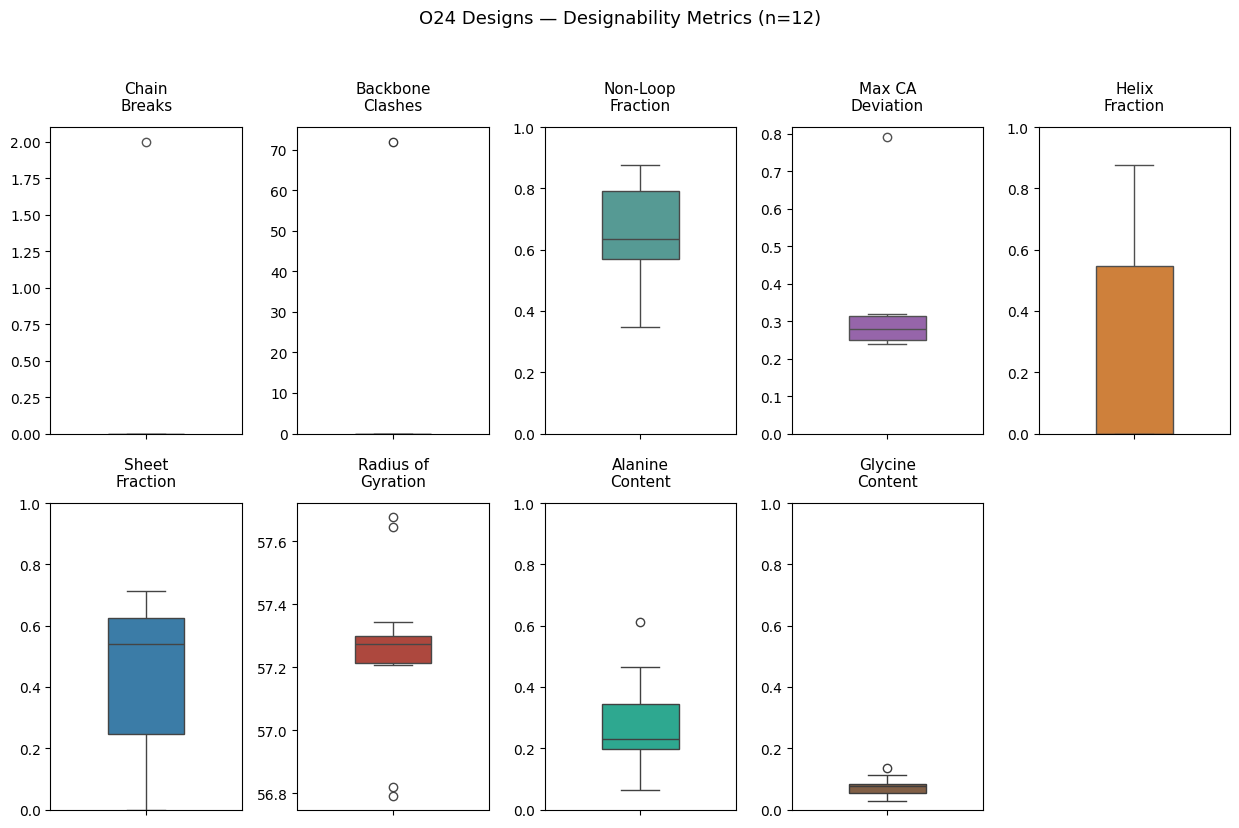
\includegraphics[width=\textwidth]{Octahedral_designability_metrics.png}
  \caption{Full designability (backbone-sanity) distributions for the octahedral
    O24 designs ($n{=}12$).}
  \label{fig:oct-des}
\end{figure}

\begin{figure}[h]
  \centering
  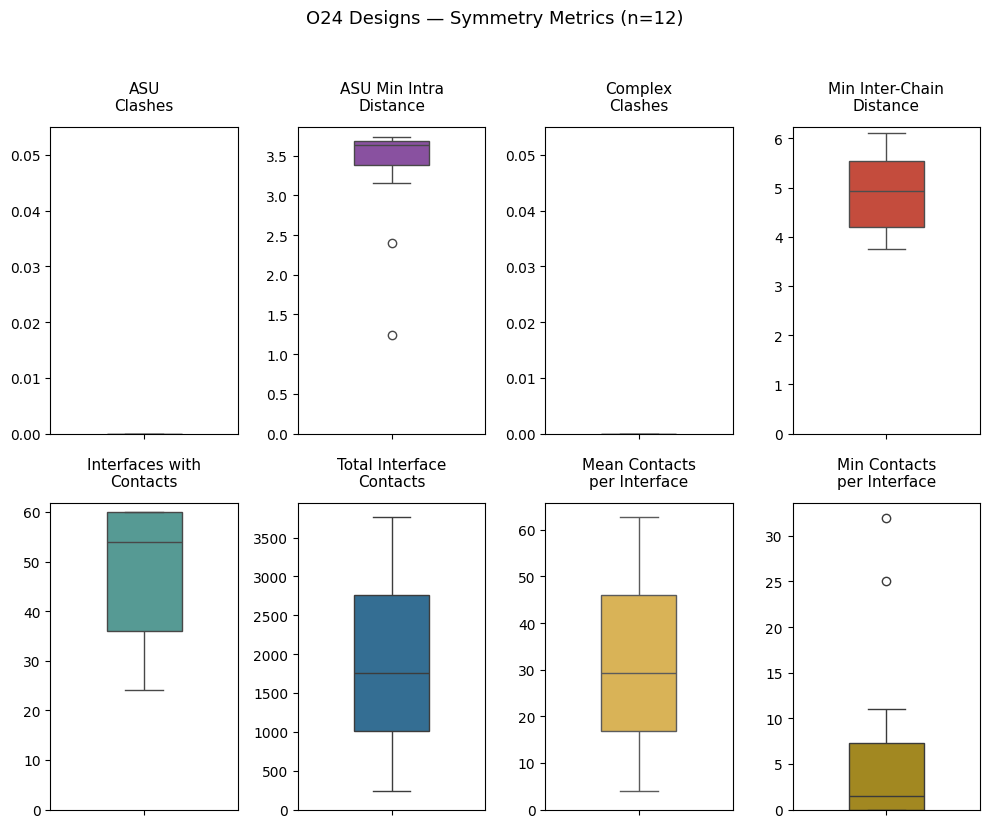
\includegraphics[width=\textwidth]{Octahedral_symmetry_metrics.png}
  \caption{Full symmetry-aware interface metric distributions for the octahedral
    O24 designs ($n{=}12$).}
  \label{fig:oct-symm}
\end{figure}

\clearpage
\section{Effect of removing the symmetry constraint}
\label{app:monstromers}

\begin{figure}[h]
  \centering
  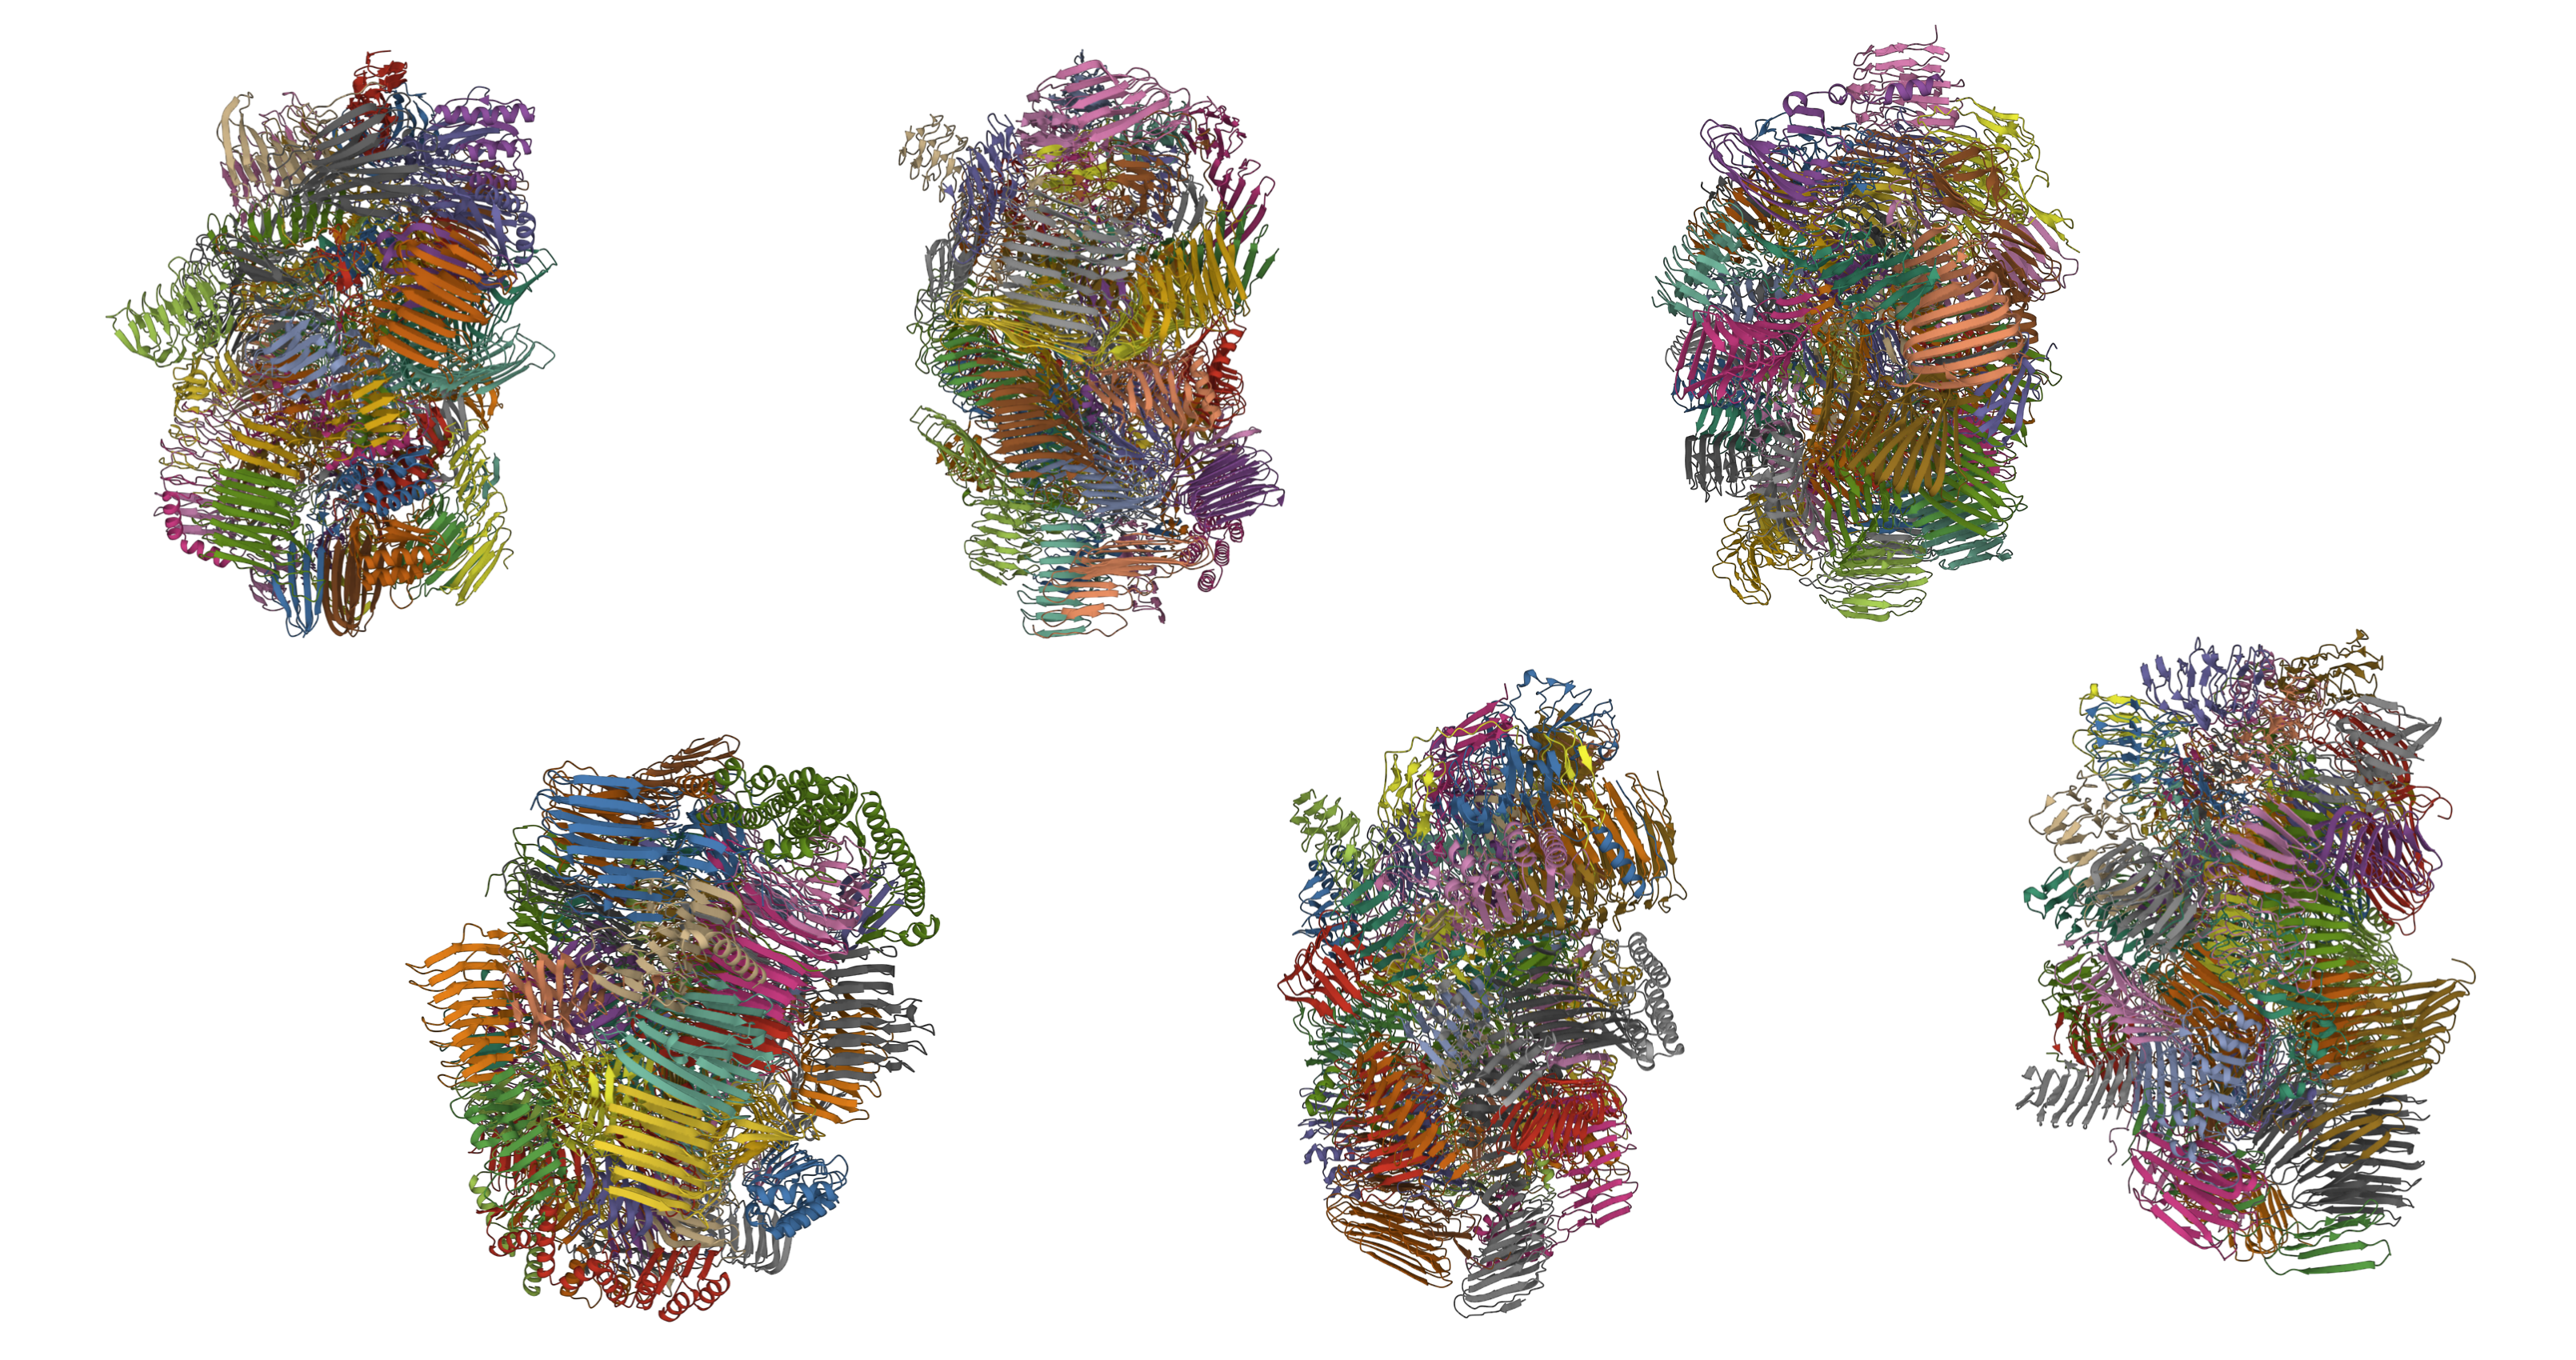
\includegraphics[width=\textwidth]{Monstromers.png}
  \caption{Six Design-CP samples at the icosahedral system size ($60$ chains
    $\times\,210$ residues $=12{,}600$ residues) generated \emph{without} a
    point-group symmetry constraint. Compared with the well-formed icosahedral
    particles of Figure~\ref{fig:icosahedral}, the unconstrained assemblies are
    malformed and non-globular, illustrating why the symmetry prior is essential in
    this beyond-crop regime.}
  \label{fig:monstromers}
\end{figure}


\end{document}
